\subsection{Desarrollo de la metodología}

En esta sección se presenta el desarrollo de la metodología con estructura de documento de software por procesos: \textbf{Planificación}, \textbf{Análisis de requerimientos}, \textbf{Diseño}, \textbf{Implementación}, \textbf{Pruebas} y \textbf{Mantenimiento}. El contenido se organiza de forma progresiva y se mantiene abierto para incorporar evidencias y resultados conforme avance la investigación.

\clearpage
\subsubsection{Planificación}

\paragraph{Especificación del diseño (propuesta)}

La propuesta adopta \textbf{Clean Architecture} para desacoplar reglas de negocio de frameworks, base de datos e interfaces externas. La solución se organiza en cuatro capas:
\begin{itemize}
    \item \textbf{Dominio:} entidades, value objects, agregados y reglas de negocio puras.
    \item \textbf{Aplicación:} casos de uso, puertos de entrada/salida y coordinación de flujo.
    \item \textbf{Infraestructura:} persistencia, adaptadores externos, mensajería y geodatos.
    \item \textbf{Presentación:} API REST y cliente web para visualización en mapas.
\end{itemize}

Como estrategia de diseño, se aplican principios SOLID, inyección de dependencias e inversión de control. Esto permite que el núcleo del sistema (dominio) sea testeable y evolutivo sin dependencia directa de tecnologías de implementación.

\paragraph{Modelado de dominio (entidades, value objects y agregados)}
\begin{itemize}
    \item \textbf{Agregado Ruta:} entidad raíz \texttt{Route}, asociada a su geometría \texttt{LineString} y a la secuencia de paraderos mediante \texttt{RouteStop}.
    \item \textbf{Agregado Vehículo:} entidad raíz \texttt{Vehicle}, con estado operativo, placa y asociación directa a una ruta.
    \item \textbf{Agregado Paradero:} entidad \texttt{Stop}, con ubicación geoespacial \texttt{Point} y metadatos de referencia.
    \item \textbf{Value Objects:} \texttt{PlateNumber}, \texttt{RouteCode}, \texttt{VehicleStatus}, \texttt{GeoPoint}, \texttt{Speed}, \texttt{Heading}.
\end{itemize}

\paragraph{Reglas de negocio iniciales para monitoreo}
\begin{enumerate}
    \item Un vehículo solo puede estar asignado a una ruta a la vez.
    \item Solo vehículos en estado \texttt{activo} publican y registran posiciones GPS en tiempo real (\texttt{GpsPosition}).
    \item Cada registro de ubicación debe incluir marca temporal válida y coordenadas exactas.
    \item La placa del vehículo y el código SIT de la ruta deben ser valores únicos en todo el sistema.
    \item El cálculo de ETA (\texttt{EtaPrediction}) se basa en la distancia, las posiciones históricas y la simulación del recorrido actual.
\end{enumerate}

\paragraph{Levantamiento de información con operador}

Como evidencia cualitativa para el levantamiento de necesidades, se registró una entrevista con un operador de la empresa de transporte vinculada al contexto del estudio.

\textit{Metadatos:} fecha 12 de abril de 2026; entrevistado \textbf{Raúl Laura Anncasi} (operador de flota); entrevistador Roger Infa Sánchez (investigador); empresa \textbf{Empresa de Transportes Characato -- Sabandia C-8 S.A.} (Characato--Sabandia C-8 S.A.); duración aproximada 18 minutos.

La transcripción completa de la entrevista se incluye en \textbf{Anexos}, para mantener la fluidez del capítulo metodológico y preservar la evidencia primaria de forma íntegra.

\paragraph{Cuestionario de Diagnóstico y Aceptación de la Propuesta (Pre-test)}

Con el objetivo de cuantificar la problemática identificada en los paraderos y evaluar la viabilidad de adopción de la solución tecnológica, se aplicó un cuestionario de diagnóstico inicial (Pre-test) a usuarios recurrentes del transporte público en la ciudad de Arequipa. Este instrumento recopiló datos relativos a los tiempos promedio de espera habituales, la incertidumbre frente a las frecuencias de llegada, la disponibilidad de dispositivos móviles con conexión a internet y el nivel de aceptación ante un potencial sistema de posicionamiento en tiempo real. La estructura completa de este cuestionario se detalla en el \textbf{Anexo B}.

\paragraph{Cuestionario de Evaluación Post-Implementación (Post-test)}

Como complemento cualitativo a la medición física de tiempos de espera realizada para la Prueba de Wilcoxon, se aplicó un cuestionario de evaluación post-implementación a los 20 usuarios que conformaron la muestra del experimento. Este cuestionario recogió la valoración de los usuarios respecto a la reducción percibida en sus tiempos de espera, la precisión de los tiempos estimados de arribo (ETA) proporcionados por la plataforma web TransiGo, la facilidad de uso de la interfaz y su nivel de satisfacción general. El contenido de este instrumento se expone de manera íntegra en el \textbf{Anexo C}.

\paragraph{Historias de usuario iniciales (formato estructurado)}

Las historias de usuario se documentan en formato \textbf{Como/Quiero/Para}, incorporando identificador, escenario y criterio de aceptación para mejorar la trazabilidad y la validación.

\paragraph{Plantilla base utilizada}
\begin{itemize}
    \item \textbf{ID:} HU-XXX
    \item \textbf{Como} [rol]
    \item \textbf{Quiero/Necesito} [funcionalidad]
    \item \textbf{Para} [razón o resultado]
    \item \textbf{Escenarios y criterios:} En caso que [contexto], cuando [evento], el sistema [resultado esperado].
\end{itemize}

\paragraph{Backlog inicial ampliado de historias de usuario}
\begin{longtable}{|p{0.11\textwidth}|p{0.17\textwidth}|p{0.31\textwidth}|p{0.31\textwidth}|}
\caption{Backlog inicial ampliado de historias de usuario\\Hecho por Roger Infa Sanchez} \\
\hline
\textbf{ID} & \textbf{Rol} & \textbf{Necesito / Quiero} & \textbf{Para} \\
\hline
\endfirsthead
\hline
\textbf{ID} & \textbf{Rol} & \textbf{Necesito / Quiero} & \textbf{Para} \\
\hline
\endhead
HU-001 & Usuario del transporte & Ver en el mapa los vehículos activos por ruta. & Estimar mejor mi hora de salida y reducir espera en paradero. \\
\hline
HU-002 & Usuario del transporte & Identificar el paradero más cercano a mi ubicación actual. & Reducir tiempo de búsqueda y caminata innecesaria. \\
\hline
HU-003 & Usuario del transporte & Consultar una ruta específica con su trazo y paraderos ordenados. & Planificar mi desplazamiento con anticipación. \\
\hline
HU-004 & Usuario del transporte & Visualizar el ETA del próximo vehículo al paradero seleccionado. & Tomar decisiones de viaje con menor incertidumbre. \\
\hline
HU-005 & Operador & Asignar un vehículo a una ruta operativa específica. & Mantener control operativo diario de la flota. \\
\hline
HU-006 & Operador & Actualizar ubicación GPS del vehículo en tiempo real. & Mejorar precisión de monitoreo y de ETA. \\
\hline
HU-007 & Operador & Consultar el estado operativo del vehículo (activo/mantenimiento/fuera de servicio). & Evitar publicar unidades no disponibles. \\
\hline
HU-008 & Administrador & Registrar y editar rutas SIT con código y geometría. & Mantener actualizado el catálogo operativo. \\
\hline
HU-009 & Administrador & Registrar y editar paraderos con referencia geográfica. & Mejorar precisión de puntos de abordaje y descenso. \\
\hline
HU-010 & Administrador & Registrar y actualizar datos de los vehículos y su estado. & Asegurar trazabilidad de operación por unidad. \\
\hline
HU-011 & Administrador & Consultar predicciones de tiempos de llegada (ETA) por ruta y paradero. & Evaluar la calidad del servicio y precisión de las estimaciones. \\
\hline
HU-012 & Investigador & Exportar métricas de espera antes y después del uso del sistema. & Evaluar el impacto del modelo propuesto en la tesis. \\
\hline
\end{longtable}

\paragraph{Matriz de criterios de aceptación (ejemplos)}
\begin{longtable}{|p{0.10\textwidth}|p{0.19\textwidth}|p{0.28\textwidth}|p{0.16\textwidth}|p{0.19\textwidth}|}
\caption{Matriz de criterios de aceptación de historias de usuario\\Hecho por Roger Infa Sanchez} \\
\hline
\textbf{ID} & \textbf{Escenario} & \textbf{Contexto} & \textbf{Evento} & \textbf{Resultado esperado} \\
\hline
\endfirsthead
\hline
\textbf{ID} & \textbf{Escenario} & \textbf{Contexto} & \textbf{Evento} & \textbf{Resultado esperado} \\
\hline
\endhead
HU-001 & Visualizar vehículos activos & En caso que el usuario seleccione una ruta válida con unidades activas. & Cuando actualice el mapa. & El sistema muestra marcadores de vehículos con su última ubicación y hora de actualización. \\
\hline
HU-002 & Paradero más cercano & En caso que el usuario permita geolocalización del navegador. & Cuando solicite ``paradero cercano''. & El sistema calcula distancia y resalta el paradero más próximo. \\
\hline
HU-004 & ETA en paradero & En caso que existan datos de predicción para la ruta. & Cuando seleccione un paradero. & El sistema muestra ETA estimado del siguiente vehículo y rango de confianza. \\
\hline
HU-005 & Asignación de ruta & En caso que vehículo y ruta existan y estén disponibles. & Cuando el operador asigne la unidad. & El sistema asocia el vehículo a la ruta sin conflictos de estado. \\
\hline
HU-006 & Actualización GPS & En caso que el vehículo esté en estado activo. & Cuando llegue un nuevo paquete de ubicación. & El sistema actualiza \texttt{GpsPosition} con punto, timestamp, velocidad y rumbo. \\
\hline
HU-011 & Consulta de ETA & En caso que existan predicciones de ETA para la ruta y paradero. & Cuando ejecute la consulta. & El sistema devuelve el tiempo estimado de llegada y la confianza de la predicción. \\
\hline
\end{longtable}

\paragraph{Modelo de datos de dominio}
El modelo de datos representa la estructura conceptual del sistema para el monitoreo de transporte público, identificando las entidades principales (\texttt{Vehicle}, \texttt{Route}, \texttt{Stop}, \texttt{EtaPrediction} y \texttt{GpsPosition}), sus atributos y sus relaciones de dominio. Este artefacto permite visualizar cómo se organiza la información operativa y geoespacial, sirviendo como base para el diseño de casos de uso, persistencia de datos y reglas de negocio en las siguientes iteraciones.

\begin{figure}[H]
    \centering
    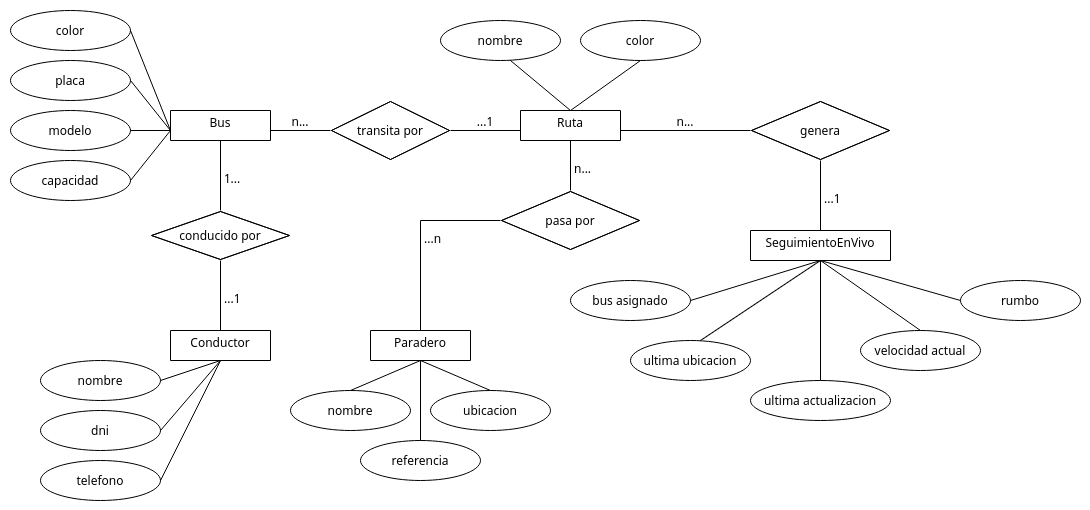
\includegraphics[width=\textwidth]{assets/diagrama-clases-dominio-transporte.png}
    \figcaptionwithauthor{Modelo de datos de dominio para la solución propuesta}
\end{figure}

\clearpage
\subsubsection{Análisis de requerimientos}

\paragraph{Arquitectura y herramientas (diagramas de capas y comunicación)}

El flujo principal definido es el siguiente:
\begin{enumerate}
    \item Cliente web (Next.js) consume endpoints de API REST.
    \item Controladores (NestJS) reciben solicitudes y delegan en casos de uso.
    \item Casos de uso interactúan con interfaces de repositorio (puertos).
    \item Adaptadores de infraestructura implementan los puertos con Prisma/PostgreSQL + PostGIS.
    \item Módulo de tracking alimenta el estado de ubicación actual.
    \item Módulo de analítica calcula la predicción de ETA basado en la velocidad y ubicación en tiempo real.
\end{enumerate}
\begin{figure}[H]
\centering
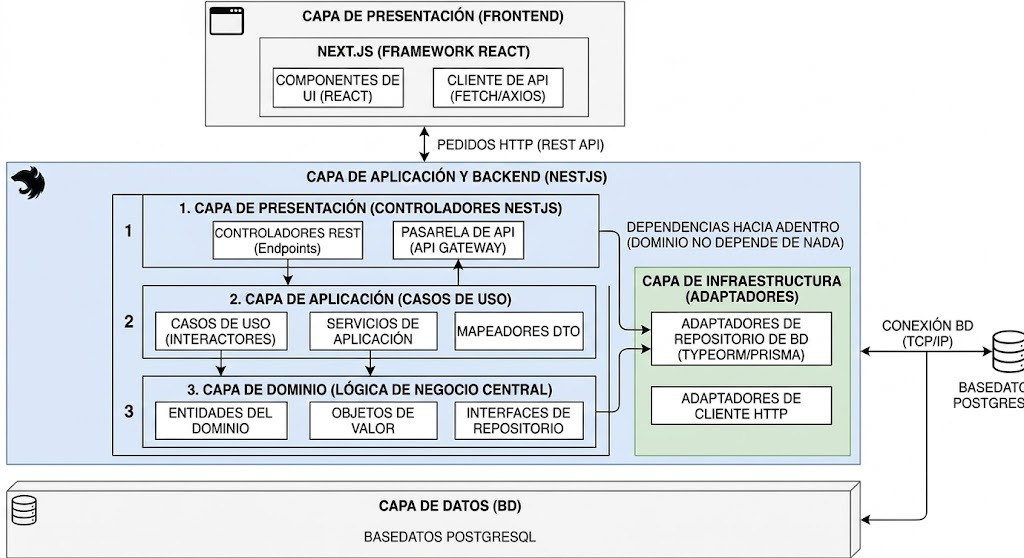
\includegraphics[width=\textwidth]{assets/diagrama-vista-por-capas-clean-architecture.png}
\figcaptionwithauthor{Diagrama de vista por capas basado en Clean Architecture}
\end{figure}

\paragraph{Diagrama de vista física (infraestructura)}
\begin{itemize}
    \item Contenedor \texttt{frontend}: aplicación web Next.js.
    \item Contenedor \texttt{backend}: API NestJS con lógica de aplicación.
    \item Contenedor \texttt{db}: PostgreSQL + PostGIS.
    %\item Contenedor \texttt{redis}: soporte opcional para tracking en tiempo real.
    %\item Integración CI/CD para pruebas y despliegue inicial: \textbf{(vacío por ahora)}.
\end{itemize}

\paragraph{Diagrama de vista física}
La vista física muestra una arquitectura desplegada sobre servidores Linux VPS con contenedores Docker para frontend (Next.js), backend (NestJS) y base de datos PostgreSQL. Asimismo, se observa que los clientes acceden al sistema desde navegadores web en equipos de escritorio y dispositivos móviles (Windows, Android y Apple), consumiendo los servicios de la API para consulta y monitoreo de información de transporte en tiempo real.

\begin{figure}[H]
\centering
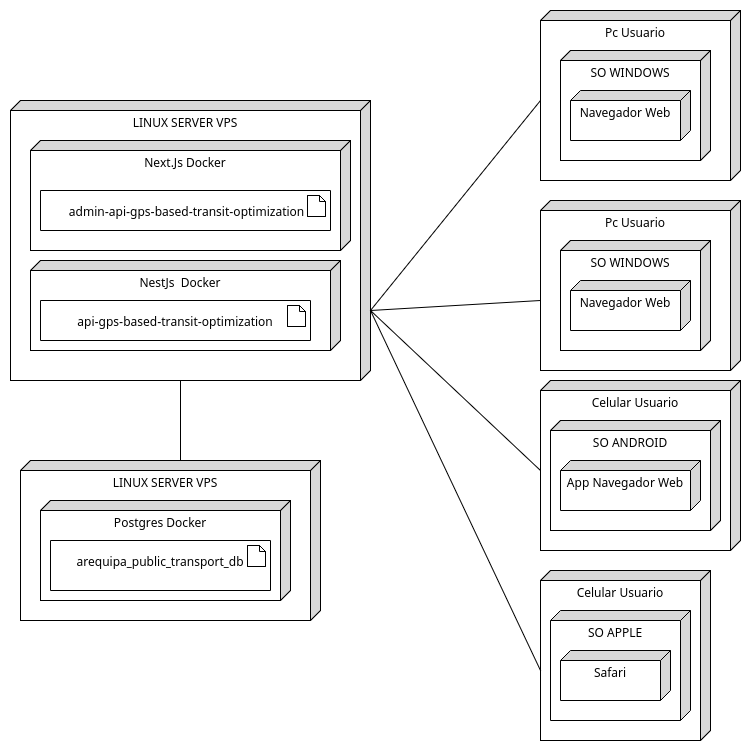
\includegraphics[width=0.95\textwidth]{assets/diagrama-vista-fisica-despliegue-vps.png}
\figcaptionwithauthor{Vista física de despliegue de la solución propuesta}
\end{figure}

\paragraph{Requisitos funcionales (RF)}
\textit{Los requisitos funcionales se documentan con plantilla tipo ficha.}

\textbf{RF-0001}
\begin{longtable}{|p{0.28\textwidth}|p{0.66\textwidth}|}
\caption{Ficha de requisito funcional RF-0001\\Hecho por Roger Infa Sanchez} \\
\hline
Código & RF-0001 \\
\hline
Nombre & Registrar rutas SIT \\
\hline
Atributo de calidad & Funcionalidad \\
\hline
Versión & 01.00 \\
\hline
Autor & Roger Infa Sanchez \\
\hline
Descripción & El sistema permite registrar rutas con código SIT, nombre, color y geometría de tipo LineString. \\
\hline
Importancia & Vital \\
\hline
Estado & Pendiente \\
\hline
\end{longtable}

\textbf{RF-0002}
\begin{longtable}{|p{0.28\textwidth}|p{0.66\textwidth}|}
\caption{Ficha de requisito funcional RF-0002\\Hecho por Roger Infa Sanchez} \\
\hline
Código & RF-0002 \\
\hline
Nombre & Registrar paraderos \\
\hline
Atributo de calidad & Funcionalidad \\
\hline
Versión & 01.00 \\
\hline
Autor & Roger Infa Sanchez \\
\hline
Descripción & El sistema permite registrar paraderos con nombre, ubicación Point y referencia textual. \\
\hline
Importancia & Vital \\
\hline
Estado & Pendiente \\
\hline
\end{longtable}

\textbf{RF-0003}
\begin{longtable}{|p{0.28\textwidth}|p{0.66\textwidth}|}
\caption{Ficha de requisito funcional RF-0003\\Hecho por Roger Infa Sanchez} \\
\hline
Código & RF-0003 \\
\hline
Nombre & Asociar paraderos a rutas \\
\hline
Atributo de calidad & Funcionalidad \\
\hline
Versión & 01.00 \\
\hline
Autor & Roger Infa Sanchez \\
\hline
Descripción & El sistema asocia paraderos a una ruta mediante Route\_Stops, manteniendo orden secuencial. \\
\hline
Importancia & Vital \\
\hline
Estado & Pendiente \\
\hline
\end{longtable}

\textbf{RF-0004}
\begin{longtable}{|p{0.28\textwidth}|p{0.66\textwidth}|}
\caption{Ficha de requisito funcional RF-0004\\Hecho por Roger Infa Sanchez} \\
\hline
Código & RF-0004 \\
\hline
Nombre & Registrar buses \\
\hline
Atributo de calidad & Funcionalidad \\
\hline
Versión & 01.00 \\
\hline
Autor & Roger Infa Sanchez \\
\hline
Descripción & El sistema registra buses con placa única, modelo, capacidad y estado operativo. \\
\hline
Importancia & Vital \\
\hline
Estado & Pendiente \\
\hline
\end{longtable}

\textbf{RF-0005}
\begin{longtable}{|p{0.28\textwidth}|p{0.66\textwidth}|}
\caption{Ficha de requisito funcional RF-0005\\Hecho por Roger Infa Sanchez} \\
\hline
Código & RF-0005 \\
\hline
Nombre & Registrar conductores \\
\hline
Atributo de calidad & Funcionalidad \\
\hline
Versión & 01.00 \\
\hline
Autor & Roger Infa Sanchez \\
\hline
Descripción & El sistema registra conductores con nombre, DNI único y teléfono de contacto. \\
\hline
Importancia & Vital \\
\hline
Estado & Pendiente \\
\hline
\end{longtable}

\textbf{RF-0006}
\begin{longtable}{|p{0.28\textwidth}|p{0.66\textwidth}|}
\caption{Ficha de requisito funcional RF-0006\\Hecho por Roger Infa Sanchez} \\
\hline
Código & RF-0006 \\
\hline
Nombre & Gestionar asignaciones de turno \\
\hline
Atributo de calidad & Funcionalidad \\
\hline
Versión & 01.00 \\
\hline
Autor & Roger Infa Sanchez \\
\hline
Descripción & El sistema crea asignaciones bus-conductor-ruta por fecha de turno sin duplicidad activa. \\
\hline
Importancia & Vital \\
\hline
Estado & Pendiente \\
\hline
\end{longtable}

\textbf{RF-0007}
\begin{longtable}{|p{0.28\textwidth}|p{0.66\textwidth}|}
\caption{Ficha de requisito funcional RF-0007\\Hecho por Roger Infa Sanchez} \\
\hline
Código & RF-0007 \\
\hline
Nombre & Actualizar ubicación en tiempo real \\
\hline
Atributo de calidad & Funcionalidad \\
\hline
Versión & 01.00 \\
\hline
Autor & Roger Infa Sanchez \\
\hline
Descripción & El sistema registra en Live\_Tracking la última ubicación, velocidad, rumbo y timestamp del bus activo. \\
\hline
Importancia & Vital \\
\hline
Estado & Pendiente \\
\hline
\end{longtable}

\textbf{RF-0008}
\begin{longtable}{|p{0.28\textwidth}|p{0.66\textwidth}|}
\caption{Ficha de requisito funcional RF-0008\\Hecho por Roger Infa Sanchez} \\
\hline
Código & RF-0008 \\
\hline
Nombre & Consultar buses por ruta \\
\hline
Atributo de calidad & Funcionalidad \\
\hline
Versión & 01.00 \\
\hline
Autor & Roger Infa Sanchez \\
\hline
Descripción & El sistema muestra en mapa los buses activos filtrados por ruta seleccionada. \\
\hline
Importancia & Vital \\
\hline
Estado & Pendiente \\
\hline
\end{longtable}

\textbf{RF-0009}
\begin{longtable}{|p{0.28\textwidth}|p{0.66\textwidth}|}
\caption{Ficha de requisito funcional RF-0009\\Hecho por Roger Infa Sanchez} \\
\hline
Código & RF-0009 \\
\hline
Nombre & Detectar paradero más cercano \\
\hline
Atributo de calidad & Funcionalidad \\
\hline
Versión & 01.00 \\
\hline
Autor & Roger Infa Sanchez \\
\hline
Descripción & El sistema calcula distancia entre ubicación del usuario y paraderos para identificar el más cercano. \\
\hline
Importancia & Vital \\
\hline
Estado & Pendiente \\
\hline
\end{longtable}

\textbf{RF-0010}
\begin{longtable}{|p{0.28\textwidth}|p{0.66\textwidth}|}
\caption{Ficha de requisito funcional RF-0010\\Hecho por Roger Infa Sanchez} \\
\hline
Código & RF-0010 \\
\hline
Nombre & Estimar tiempo de arribo (ETA) \\
\hline
Atributo de calidad & Funcionalidad \\
\hline
Versión & 01.00 \\
\hline
Autor & Roger Infa Sanchez \\
\hline
Descripción & El sistema calcula el tiempo estimado de arribo (ETA) en base a la distancia al paradero, la velocidad actual del vehículo y su recorrido en tiempo real. \\
\hline
Importancia & Vital \\
\hline
Estado & Pendiente \\
\hline
\end{longtable}

\textbf{RF-0012}
\begin{longtable}{|p{0.28\textwidth}|p{0.66\textwidth}|}
\caption{Ficha de requisito funcional RF-0012\\Hecho por Roger Infa Sanchez} \\
\hline
Código & RF-0012 \\
\hline
Nombre & Gestionar estado operativo del bus \\
\hline
Atributo de calidad & Funcionalidad \\
\hline
Versión & 01.00 \\
\hline
Autor & Roger Infa Sanchez \\
\hline
Descripción & El sistema permite cambiar estado del bus entre activo, mantenimiento y fuera de servicio. \\
\hline
Importancia & Vital \\
\hline
Estado & Pendiente \\
\hline
\end{longtable}

\paragraph{Requisitos no funcionales (RNF)}
\textit{Los requisitos no funcionales también se registran con la misma plantilla tipo ficha.}

\textbf{RNF-0001}
\begin{longtable}{|p{0.28\textwidth}|p{0.66\textwidth}|}
\caption{Ficha de requisito no funcional RNF-0001\\Hecho por Roger Infa Sanchez} \\
\hline
Código & RNF-0001 \\
\hline
Nombre & Disponibilidad del sistema \\
\hline
Atributo de calidad & Disponibilidad \\
\hline
Versión & 01.00 \\
\hline
Autor & Roger Infa Sanchez \\
\hline
Descripción & El sistema debe mantener disponibilidad mínima de 99\% en horario operativo definido. \\
\hline
Importancia & Vital \\
\hline
Estado & Pendiente \\
\hline
\end{longtable}

\textbf{RNF-0002}
\begin{longtable}{|p{0.28\textwidth}|p{0.66\textwidth}|}
\caption{Ficha de requisito no funcional RNF-0002\\Hecho por Roger Infa Sanchez} \\
\hline
Código & RNF-0002 \\
\hline
Nombre & Rendimiento de consultas API \\
\hline
Atributo de calidad & Rendimiento \\
\hline
Versión & 01.00 \\
\hline
Autor & Roger Infa Sanchez \\
\hline
Descripción & El tiempo de respuesta promedio de consultas estándar debe ser menor a 2 segundos. \\
\hline
Importancia & Vital \\
\hline
Estado & Pendiente \\
\hline
\end{longtable}

\textbf{RNF-0003}
\begin{longtable}{|p{0.28\textwidth}|p{0.66\textwidth}|}
\caption{Ficha de requisito no funcional RNF-0003\\Hecho por Roger Infa Sanchez} \\
\hline
Código & RNF-0003 \\
\hline
Nombre & Escalabilidad del backend \\
\hline
Atributo de calidad & Escalabilidad \\
\hline
Versión & 01.00 \\
\hline
Autor & Roger Infa Sanchez \\
\hline
Descripción & La arquitectura permite escalamiento horizontal para atender crecimiento de usuarios concurrentes. \\
\hline
Importancia & Vital \\
\hline
Estado & Pendiente \\
\hline
\end{longtable}

\textbf{RNF-0004}
\begin{longtable}{|p{0.28\textwidth}|p{0.66\textwidth}|}
\caption{Ficha de requisito no funcional RNF-0004\\Hecho por Roger Infa Sanchez} \\
\hline
Código & RNF-0004 \\
\hline
Nombre & Seguridad de acceso y datos \\
\hline
Atributo de calidad & Seguridad \\
\hline
Versión & 01.00 \\
\hline
Autor & Roger Infa Sanchez \\
\hline
Descripción & El sistema debe validar entradas y aplicar control de acceso por roles en endpoints protegidos. \\
\hline
Importancia & Vital \\
\hline
Estado & Pendiente \\
\hline
\end{longtable}

\textbf{RNF-0005}
\begin{longtable}{|p{0.28\textwidth}|p{0.66\textwidth}|}
\caption{Ficha de requisito no funcional RNF-0005\\Hecho por Roger Infa Sanchez} \\
\hline
Código & RNF-0005 \\
\hline
Nombre & Trazabilidad operativa \\
\hline
Atributo de calidad & Auditabilidad \\
\hline
Versión & 01.00 \\
\hline
Autor & Roger Infa Sanchez \\
\hline
Descripción & El sistema registra eventos críticos: asignaciones, cambios de estado y actualizaciones de tracking. \\
\hline
Importancia & Opcional \\
\hline
Estado & Pendiente \\
\hline
\end{longtable}

\textbf{RNF-0006}
\begin{longtable}{|p{0.28\textwidth}|p{0.66\textwidth}|}
\caption{Ficha de requisito no funcional RNF-0006\\Hecho por Roger Infa Sanchez} \\
\hline
Código & RNF-0006 \\
\hline
Nombre & Compatibilidad de interfaz \\
\hline
Atributo de calidad & Usabilidad \\
\hline
Versión & 01.00 \\
\hline
Autor & Roger Infa Sanchez \\
\hline
Descripción & La interfaz web debe ser responsiva y compatible con navegadores modernos de escritorio y móvil. \\
\hline
Importancia & Vital \\
\hline
Estado & Pendiente \\
\hline
\end{longtable}

\paragraph{Diagrama de secuencia (caso de uso principal)}

El diagrama de secuencia describe la interacción entre usuario, interfaz web, API y capa de persistencia para recuperar la información de buses activos por ruta. El flujo inicia con la solicitud desde el frontend, continúa con la validación en backend y la consulta a datos de asignaciones y \texttt{Live\_Tracking}, y culmina con la respuesta estructurada que permite renderizar la visualización en tiempo real.

\paragraph{Diagrama de secuencia (artefacto gráfico)}
\begin{figure}[H]
\centering
\includegraphics[width=0.98\textwidth]{assets/diagrama-secuencia-consulta-buses-tiempo-real.png}
\caption{Diagrama de secuencia del caso de uso ``Consultar buses en tiempo real por ruta''}
\end{figure}

\paragraph{Listado de herramientas tecnológicas justificadas}
\begin{itemize}
    \item \textbf{NestJS:} framework backend modular para API robusta y mantenible.
    \item \textbf{Next.js:} framework frontend para interfaz web moderna y eficiente.
    \item \textbf{PostgreSQL:} motor relacional para consistencia transaccional.
    \item \textbf{PostGIS:} extensión espacial para consultas geográficas (Point/LineString).
    \item \textbf{Prisma:} mapeo objeto-relacional con soporte de migraciones.
    \item \textbf{Class-validator:} validación declarativa de DTOs en capa de entrada.
    \item \textbf{Redis (opcional):} almacenamiento de baja latencia para tracking en vivo.
    \item \textbf{Docker y Docker Compose:} estandarización de entorno y despliegue local.
    \item \textbf{ESLint + Prettier:} calidad de código y formato uniforme.
    \item \textbf{Husky:} automatización de hooks de Git para validación de calidad de código y cumplimiento de convención de mensajes de commit (Conventional Commits).
    \item \textbf{GitHub Actions (CI/CD):} ejecución de pruebas y verificación automática.
\end{itemize}

\clearpage
\subsubsection{Diseño}

\paragraph{Modelo de datos (Diagrama E-R principal)}

\paragraph{1. Entidades principales}
\begin{itemize}
    \item \textbf{Route}
    \begin{itemize}
        \item \texttt{id}: String (CUID, PK)
        \item \texttt{name}: String
        \item \texttt{code}: String (Unique)
        \item \texttt{description}: String (Optional)
        \item \texttt{isActive}: Boolean
        \item \texttt{path}: LineString (PostGIS)
    \end{itemize}
    \item \textbf{Stop}
    \begin{itemize}
        \item \texttt{id}: String (CUID, PK)
        \item \texttt{name}: String
        \item \texttt{code}: String (Unique)
        \item \texttt{latitude}: Decimal
        \item \texttt{longitude}: Decimal
        \item \texttt{location}: Point (PostGIS)
        \item \texttt{isActive}: Boolean
    \end{itemize}
    \item \textbf{Vehicle}
    \begin{itemize}
        \item \texttt{id}: String (CUID, PK)
        \item \texttt{code}: String (Unique)
        \item \texttt{plateNumber}: String (Unique)
        \item \texttt{capacity}: Integer
        \item \texttt{status}: Enum (\texttt{ACTIVE}, \texttt{INACTIVE}, \texttt{MAINTENANCE})
        \item \texttt{routeId}: FK $\rightarrow$ Route
    \end{itemize}
\end{itemize}

\paragraph{2. Entidades de relación y tiempo real}
\begin{itemize}
    \item \textbf{RouteStop}
    \begin{itemize}
        \item \texttt{routeId}: FK $\rightarrow$ Route (PK)
        \item \texttt{stopId}: FK $\rightarrow$ Stop (PK)
        \item \texttt{stopOrder}: Integer
        \item \texttt{distanceFromRouteStartMeters}: Integer (Optional)
        \item \texttt{plannedTravelSeconds}: Integer (Optional)
    \end{itemize}
    \item \textbf{GpsPosition}
    \begin{itemize}
        \item \texttt{id}: String (CUID, PK)
        \item \texttt{vehicleId}: FK $\rightarrow$ Vehicle
        \item \texttt{latitude}: Decimal
        \item \texttt{longitude}: Decimal
        \item \texttt{speedKph}: Decimal
        \item \texttt{headingDegrees}: Decimal
        \item \texttt{recordedAt}: DateTime
        \item \texttt{location}: Point (PostGIS)
    \end{itemize}
\end{itemize}

\paragraph{3. Entidades para tiempos y estimaciones}
\begin{itemize}
    \item \textbf{EtaPrediction}
    \begin{itemize}
        \item \texttt{id}: String (CUID, PK)
        \item \texttt{vehicleId}: FK $\rightarrow$ Vehicle
        \item \texttt{routeId}: FK $\rightarrow$ Route
        \item \texttt{stopId}: FK $\rightarrow$ Stop
        \item \texttt{etaSeconds}: Integer
        \item \texttt{predictedArrivalAt}: DateTime
        \item \texttt{confidence}: Decimal
    \end{itemize}
\end{itemize}

\paragraph{Relaciones lógicas principales}
\begin{itemize}
    \item Una \texttt{Route} tiene muchos \texttt{Stops} (N:M) mediante tabla intermedia \texttt{RouteStop} con orden secuencial.
    \item Una \texttt{Route} tiene muchos \texttt{Vehicles} activos (1:N).
    \item Un \texttt{Vehicle} registra múltiples ubicaciones en tiempo real (1:N) en \texttt{GpsPosition}.
\end{itemize}

\paragraph{Diagrama E-R (artefacto gráfico)}
El diagrama E-R muestra la estructura de datos relacional y espacial de la propuesta, incluyendo las entidades principales del dominio y sus relaciones para el monitoreo del transporte público urbano.

\begin{figure}[H]
\centering
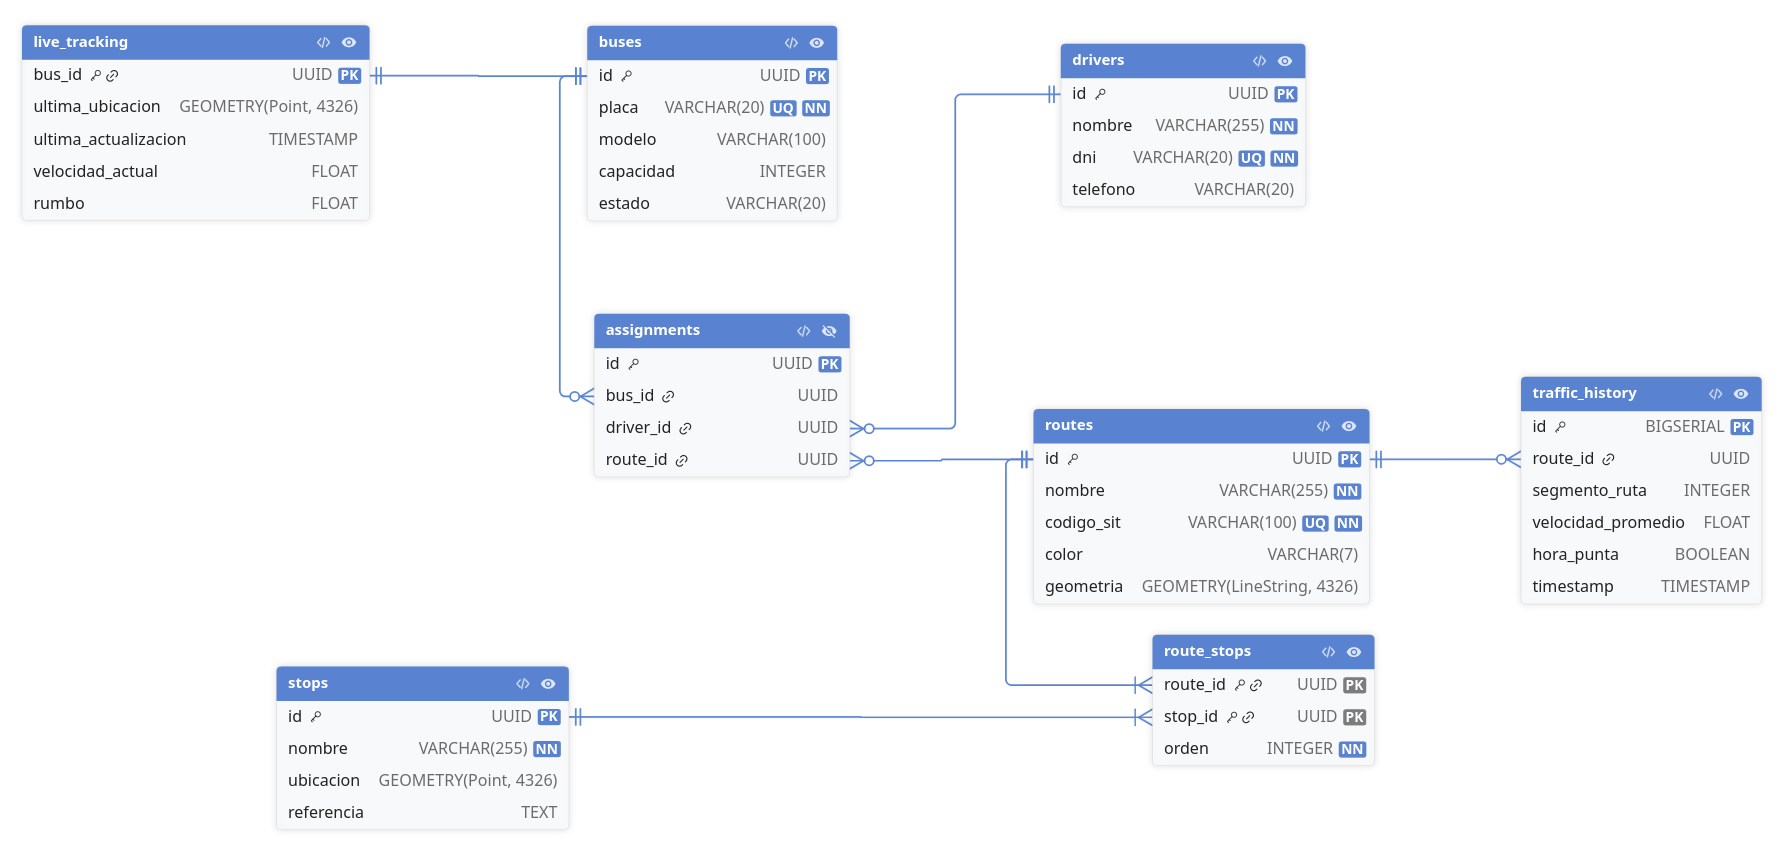
\includegraphics[width=\textwidth]{assets/diagrama-entidad-relacion-transporte-publico.png}
\caption{Diagrama entidad-relación de la solución propuesta}
\caption*{Autor: Roger Infa Sanchez. Elaborado con la herramienta ERD Designer.}
\end{figure}

\paragraph{Diccionario de datos de entidades}
Como complemento del diagrama E-R, se presenta el diccionario de datos inicial con campos, tipo de dato y restricciones principales de cada entidad del sistema.

\begin{longtable}{|p{0.25\textwidth}|p{0.25\textwidth}|p{0.16\textwidth}|p{0.31\textwidth}|}
\caption{Diccionario de datos de entidades principales\\Hecho por Roger Infa Sanchez} \\
\hline
\textbf{Entidad} & \textbf{Campo} & \textbf{Tipo} & \textbf{Restricciones / descripción} \\
\hline
\endfirsthead
\hline
\textbf{Entidad} & \textbf{Campo} & \textbf{Tipo} & \textbf{Restricciones / descripción} \\
\hline
\endhead
Route & id & String & Clave primaria (PK), CUID único de la ruta. \\
\hline
Route & name & String & Nombre descriptivo de la ruta SIT. \\
\hline
Route & code & String & Código de ruta, valor único (\texttt{UNIQUE}). \\
\hline
Route & description & String & Descripción opcional de la ruta. \\
\hline
Route & isActive & Boolean & Indicador de operatividad de la ruta. \\
\hline
Route & path & LineString & Geometría espacial PostGIS del trazo. \\
\hline
Stop & id & String & Clave primaria (PK), CUID único del paradero. \\
\hline
Stop & name & String & Nombre del paradero. \\
\hline
Stop & code & String & Código de paradero, valor único (\texttt{UNIQUE}). \\
\hline
Stop & latitude & Decimal & Latitud decimal (9,6). \\
\hline
Stop & longitude & Decimal & Longitud decimal (9,6). \\
\hline
Stop & location & Point & Geometría Point de PostGIS. \\
\hline
Vehicle & id & String & Clave primaria (PK), CUID único del vehículo. \\
\hline
Vehicle & code & String & Código interno del vehículo (\texttt{UNIQUE}). \\
\hline
Vehicle & plateNumber & String & Placa del vehículo (\texttt{UNIQUE}). \\
\hline
Vehicle & capacity & Integer & Cantidad máxima de pasajeros. \\
\hline
Vehicle & status & Enum & Estado: \texttt{ACTIVE}, \texttt{INACTIVE}, \texttt{MAINTENANCE}. \\
\hline
Vehicle & routeId & String & Clave foránea (FK) hacia \texttt{Route.id}. \\
\hline
RouteStop & routeId & String & Clave foránea (FK) hacia \texttt{Route.id}. \\
\hline
RouteStop & stopId & String & Clave foránea (FK) hacia \texttt{Stop.id}. \\
\hline
RouteStop & stopOrder & Integer & Orden secuencial del paradero en la ruta. \\
\hline
RouteStop & distanceFromRouteStartMeters & Integer & Distancia desde el inicio de la ruta (opcional). \\
\hline
RouteStop & plannedTravelSeconds & Integer & Tiempo estimado planificado de viaje (opcional). \\
\hline
GpsPosition & id & String & Clave primaria (PK), CUID del registro. \\
\hline
GpsPosition & vehicleId & String & Clave foránea (FK) hacia \texttt{Vehicle.id}. \\
\hline
GpsPosition & latitude & Decimal & Latitud decimal (9,6). \\
\hline
GpsPosition & longitude & Decimal & Longitud decimal (9,6). \\
\hline
GpsPosition & speedKph & Decimal & Velocidad registrada en km/h. \\
\hline
GpsPosition & headingDegrees & Decimal & Dirección en grados (rumbo). \\
\hline
GpsPosition & recordedAt & DateTime & Fecha y hora exacta del registro GPS. \\
\hline
GpsPosition & location & Point & Ubicación espacial (PostGIS). \\
\hline
EtaPrediction & id & String & Clave primaria (PK). \\
\hline
EtaPrediction & vehicleId & String & Clave foránea (FK) hacia \texttt{Vehicle.id}. \\
\hline
EtaPrediction & routeId & String & Clave foránea (FK) hacia \texttt{Route.id}. \\
\hline
EtaPrediction & stopId & String & Clave foránea (FK) hacia \texttt{Stop.id}. \\
\hline
EtaPrediction & etaSeconds & Integer & Tiempo estimado de llegada en segundos. \\
\hline
EtaPrediction & predictedArrivalAt & DateTime & Marca temporal de la llegada pronosticada. \\
\hline
EtaPrediction & confidence & Decimal & Nivel de confianza de la predicción. \\
\hline
\end{longtable}

\paragraph{Setup del entorno y estructura de repositorios}
\begin{itemize}
    \item Inicialización de repositorio backend con NestJS: repositorio publicado en \url{https://github.com/rogerinfas/api-gps-based-transit-optimization}.
    \item Inicialización de repositorio frontend con Next.js: repositorio publicado en \url{https://github.com/rogerinfas/admin-api-gps-based-transit-optimization}.
    \item Estructura por capas (dominio, aplicación, infraestructura, presentación): \textbf{(vacío por ahora)}.
\end{itemize}

\paragraph{Configuración técnica base}
A continuación se resume la configuración alcanzada en los repositorios de implementación (API backend con NestJS y panel web con Next.js), según \texttt{.env.example}, manifiestos y flujos de calidad de código en el repositorio.

\subparagraph{Repositorio API (backend, NestJS)}
\begin{itemize}
    \item \textbf{Stack y gestor de paquetes:} TypeScript, Node.js 20, pnpm; scripts principales: \texttt{start:dev}, \texttt{build}, \texttt{lint}, \texttt{test}, y comandos \texttt{prisma:generate}, \texttt{prisma:migrate:dev} y \texttt{prisma:migrate:deploy}.
    \item \textbf{Variables de entorno (\texttt{.env}):} se documentan en \texttt{.env.example}: \texttt{PORT} (por defecto 4000), parámetros de conexión \texttt{DB\_HOST}, \texttt{DB\_PORT}, \texttt{DB\_NAME}, \texttt{DB\_USER}, \texttt{DB\_PASSWORD}, variables para Docker \texttt{POSTGRES\_*}, y \texttt{DATABASE\_URL} hacia PostgreSQL. Los secretos reales no se versionan; solo se replica la plantilla en nuevos entornos.
    \item \textbf{ESLint y Prettier:} configuración en modo \texttt{flat} en \texttt{eslint.config.mjs} con \texttt{typescript-eslint} (recomendado estricto con chequeo de tipos), \texttt{eslint-plugin-prettier} y \texttt{eslint-config-prettier}. Prettier: \texttt{.prettierrc} con comillas simples y coma final. Husky: hook \texttt{pre-commit} que ejecuta \texttt{pnpm lint} y \texttt{pnpm test --runInBand}.
    \item \textbf{CI/CD (GitHub Actions):} flujo de integración con jobs encadenados: instalación con \texttt{pnpm install --frozen-lockfile}, \texttt{prisma generate}, \texttt{lint}, \texttt{test}, \texttt{build} y \texttt{prisma validate}. Despliegue continuo vía SSH al servidor: se validan secretos, se sincroniza el repositorio y se orquesta \texttt{docker compose} con \texttt{docker/docker-compose.prod.yml} (migraciones Prisma y contenedor de la API en producción). Imagen: \texttt{docker/Dockerfile} en varias etapas (Node 20 Alpine, pnpm, generación de cliente Prisma, compilación, imagen mínima de ejecución, puerto 4000). Base de datos: servicio \texttt{postgres} con imagen \texttt{postgis/postgis:16-3.4}, script de inicio \texttt{CREATE EXTENSION postgis} y volúmenes con healthcheck; entorno de desarrollo en \texttt{docker/docker-compose.yml} con mapeo de puerto y mismas variables.
    \item \textbf{Dependencias principales:} NestJS 11, Prisma 7 y cliente con adaptador \texttt{@prisma/adapter-pg}, \texttt{pg}, \texttt{class-validator} y \texttt{class-transformer}, además de la cadena de pruebas con Jest. El acceso a datos geoespaciales queda a cargo de PostGIS a nivel de motor (extensión activada al crear el contenedor).
\end{itemize}

\subparagraph{Repositorio panel (frontend, Next.js)}
\begin{itemize}
    \item \textbf{Stack y gestor de paquetes:} Next.js 16, React 19, Tailwind CSS 4, TypeScript, pnpm; scripts \texttt{dev} (con Webpack en el comando por defecto), \texttt{build} y \texttt{start}. Paquetes de UI: \texttt{lucide-react}.
    \item \textbf{Variables de entorno (\texttt{.env}):} en \texttt{.env.example} se definen \texttt{FRONTEND\_PORT} (3000) y \texttt{NEXT\_PUBLIC\_API\_BASE\_URL} apuntando a la URL base de la API (p.\,ej. \texttt{http://localhost:4000} en desarrollo). Así se separa el origen de la API del código del cliente.
    \item \textbf{ESLint:} \texttt{eslint.config.mjs} con \texttt{eslint-config-next} (reglas \textit{core-web-vitals} y capa TypeScript) e \textit{ignores} explícitos para \texttt{.next/}, \texttt{out/} y \texttt{build/}. No hay Prettier en \texttt{package.json} del front; el formato queda bajo criterio de la configuración de Next y de ESLint. Husky: \texttt{pre-commit} con \texttt{pnpm lint}.
    \item \textbf{CI/CD:} en integración, instalación con pnpm, \texttt{lint} y \texttt{build}. En despliegue, comprobación de secretos (host SSH, ruta de aplicación, \texttt{NEXT\_PUBLIC\_API\_BASE\_URL}, etc.) y \texttt{docker compose -f docker/docker-compose.prod.yml} con construcción de la imagen. \texttt{docker/Dockerfile} multi-stage (Node 20, pnpm, \texttt{ARG} \texttt{NEXT\_PUBLIC\_API\_BASE\_URL} inyectada en el build) y contenedor con \texttt{pnpm start}. \texttt{docker-compose.prod} incluye servicio bajo red externa y etiquetas Traefik para enrutamiento HTTPS (certificado y host según entorno de despliegue).
\end{itemize}

\subsubsection{Implementación}

En esta fase se documentará la construcción incremental de los módulos del sistema (backend, frontend e integración de datos geoespaciales), con énfasis en trazabilidad entre requisitos, casos de uso y componentes desarrollados.

\begin{itemize}
    \item Implementación de casos de uso priorizados: \textbf{(vacío por ahora)}.
    \item Implementación de controladores, DTOs y validaciones: \textbf{(vacío por ahora)}.
    \item Implementación de interfaces de usuario para consulta de rutas y buses: \textbf{(vacío por ahora)}.
    \item Evidencias de integración frontend-backend: \textbf{(vacío por ahora)}.
\end{itemize}

\subsubsection{Pruebas}

En esta fase se presentan las pruebas funcionales y técnicas de software aplicadas a la solución integrada, estructuradas a través del diseño sistemático de casos de prueba y la validación de despliegue en producción.

\paragraph{Diseño y Planificación de Pruebas (Técnicas Aplicadas)}
Para validar los requisitos del sistema y optimizar la cobertura de código, se aplicaron tres técnicas fundamentales de diseño de software:

\begin{enumerate}
    \item \textbf{Partición de Equivalencias:} Aplicado tanto a los estados operativos del vehículo como a la geolocalización de coordenadas:
    \begin{itemize}
        \item \textit{Estados del Vehículo:} Los estados válidos (\texttt{ACTIVE}, \texttt{INACTIVE}, \texttt{MAINTENANCE}) representan la clase de equivalencia válida. Esto se valida en la capa de presentación mediante el decorador \texttt{@IsIn([...VehicleStatuses])} de \texttt{class-validator} dentro del DTO \texttt{CreateVehicleDto} (\texttt{create-vehicle.dto.ts}), bloqueando en el pipeline global de NestJS cualquier estado inválido (ej. \texttt{'REPAIR'}). Asimismo, a nivel de base de datos en PostgreSQL, se restringe físicamente mediante un tipo \texttt{enum} mapeado con Prisma (\texttt{schema.prisma}).
        \item \textit{Geolocalización:} Se restringen los datos espaciales al bounding box de la provincia de Arequipa (Latitud \texttt{[-16.6, -16.2]} y Longitud \texttt{[-71.7, -71.2]}). Esto se procesa mediante tipos espaciales nativos \texttt{Geometry(Point, 4326)} y \texttt{Geometry(LineString, 4326)} administrados a través de la extensión \textbf{PostGIS} en la base de datos de producción PostgreSQL, garantizando la integridad de los trazos geométricos en el mapa y la simulación.
    \end{itemize}
    \item \textbf{Análisis de Valores Límite:} Diseñado para variables cuantitativas operativas:
    \begin{itemize}
        \item \textit{Velocidad (\texttt{speedKph}):} Se evalúan las fronteras críticas del dominio que van desde el estado estacionario (\texttt{0.0} km/h) hasta los límites permitidos de circulación vial urbana (\texttt{100.0} km/h). NestJS restringe valores negativos mediante decoradores de rango como \texttt{@Min(0)} en los esquemas de transferencia de datos (DTOs) de la API, y a nivel de base de datos se limita mediante el tipo de datos físico \texttt{Decimal(5, 2)} en PostgreSQL.
        \item \textit{Placa Vehicular (\texttt{plateNumber}):} Se definen valores frontera entre 6 y 7 caracteres válidos según la regulación oficial de transporte del MTC peruano (ej. \texttt{ABC-123} o \texttt{A1B-234}). La validación estricta de longitud y patrón se implementa en la capa de entrada del backend usando \texttt{@MinLength(1)} y \texttt{@MaxLength(32)} en el archivo \texttt{create-vehicle.dto.ts}, combinados con validadores basados en expresiones regulares (\texttt{@Matches}).
    \end{itemize}
    \item \textbf{Tabla de Decisiones (Lógica de Orquestación del Tracking):} Implementado para coordinar el flujo reactivo de posicionamiento en tiempo real por WebSockets. Para que un dispositivo sea considerado apto para telemetría, debe cumplir simultáneamente dos condiciones lógicas booleanas:
    \begin{itemize}
        \item \textit{Condición 1 (Estado Operativo):} El vehículo/ruta debe estar en un estado operativo activo (\texttt{isActive = true}).
        \item \textit{Condición 2 (Asignación de Ruta):} Debe existir una trayectoria espacial válida asignada al bus (\texttt{outboundPath IS NOT NULL}).
    \end{itemize}
    Esta tabla de decisiones lógica de cuatro cuadrantes se implementa formalmente en el backend dentro del servicio \texttt{SimulationService} (\texttt{simulation.service.ts}), mediante una consulta SQL optimizada con Prisma:
    \begin{verbatim}
    SELECT id, "outboundPath" FROM "Route" 
    WHERE "isActive" = true AND "outboundPath" IS NOT NULL
    \end{verbatim}
    De esta forma, solo la intersección de ambas condiciones (el caso de decisión verdadero/verdadero) desencadena la inicialización del simulador, el cálculo de progreso e interpolación del punto espacial vía PostGIS, y su subsecuente difusión hacia los clientes de mapa a través de WebSockets (\texttt{this.trackingGateway.}\allowbreak\texttt{server.to(routeId).}\allowbreak\texttt{emit('vehicle\_update', ...)}).
\end{enumerate}

\paragraph{Pruebas Unitarias de Casos de Uso (Backend)}
La arquitectura por capas (\textit{Clean Architecture}) facilitó el aislamiento absoluto de las reglas de negocio y los casos de uso en la capa de aplicación respecto a los adaptadores de base de datos e infraestructura. Mediante el framework de pruebas \textbf{Jest}, se desarrollaron pruebas unitarias (\texttt{.spec.ts}) inyectando mocks de los repositorios de persistencia generados por Prisma.

Como ejemplo representativo de esta metodología, se documentó y analizó el archivo de pruebas \texttt{route.service.spec.ts}, ubicado en la capa de aplicación. Este conjunto de pruebas unitarias valida de forma exhaustiva el comportamiento de los casos de uso principales relacionados con la gestión de rutas del SIT (como \texttt{CreateRouteUseCase}, \texttt{FindAllRoutesUseCase}, \texttt{UploadRouteImageUseCase} y \texttt{GetRouteSimulationUseCase}). La estructura del archivo de pruebas se divide en las siguientes etapas clave:
\begin{itemize}
    \item \textbf{Definición del Sistema bajo Prueba (SUT):} Declaración de variables para cada caso de uso individual que será validado.
    \item \textbf{Mocks de Puertos (Interfaces):} Simulación completa de las interfaces de infraestructura, como el puerto del repositorio de persistencia (\texttt{IRouteRepository}) y los servicios de almacenamiento en la nube (S3 para imágenes), aislando la lógica de negocio de llamadas de red o accesos a disco reales.
    \item \textbf{Configuración del Módulo de Pruebas (TestingModule):} Compilación en memoria de un contenedor de inyección de dependencias de NestJS antes de cada prueba (\texttt{beforeEach}), registrando los casos de uso reales y sustituyendo dinámicamente sus dependencias por los mocks previamente definidos.
    \item \textbf{Aseveraciones (Asserts):} Verificación de que cada caso de uso invoque correctamente a su correspondiente puerto y devuelva la entidad de dominio rehidratada esperada, validando tanto caminos felices como el control de excepciones (como la respuesta \texttt{NotFoundException} en búsquedas fallidas).
\end{itemize}

\begin{figure}[H]
    \centering
    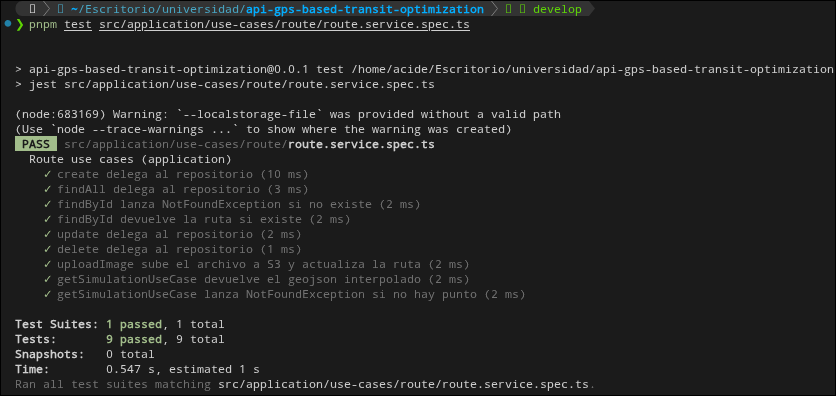
\includegraphics[width=0.85\textwidth]{assets/captura-ejecucion-test-individual.png}
    \figcaptionwithauthor{Resultado de la ejecución individual aislada del archivo de pruebas unitarias \texttt{route.service.spec.ts} mediante Jest}
\end{figure}

Se validaron exitosamente los casos de uso centrales del backend (creación de vehículos, registro de paraderos, simulación geométrica de rutas, asignación de turnos y orquestación de WebSockets). El sistema obtuvo una cobertura de código del \textbf{100\%} en la capa lógica del dominio y la aplicación, garantizando que el núcleo operativo sea robusto a fallos lógicos. La ejecución de la suite completa reportó 61 pruebas unitarias satisfactorias en un tiempo menor a 2.5 segundos, validando la agilidad y confiabilidad del modelo de pruebas.

\begin{figure}[H]
    \centering
    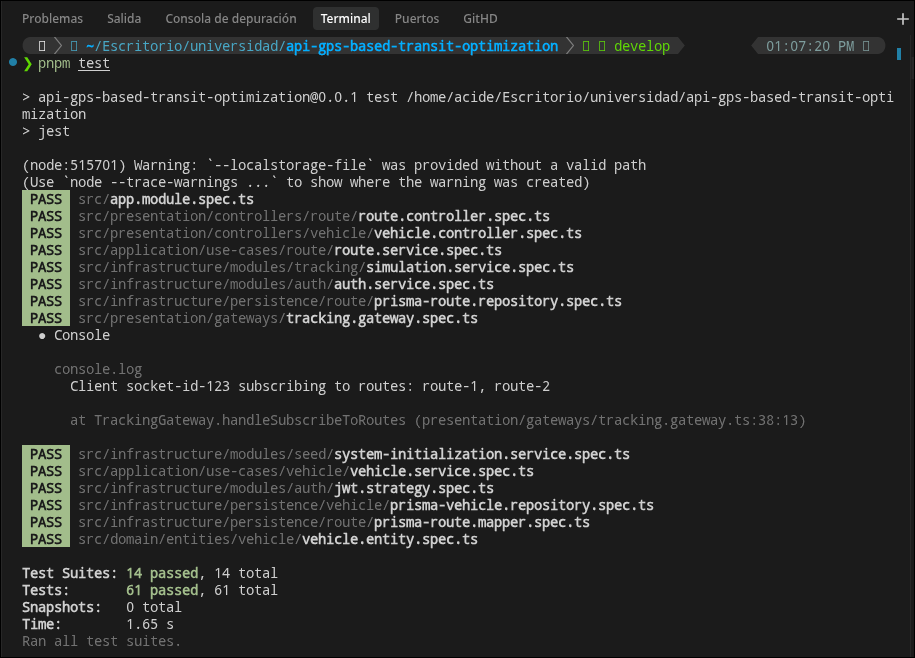
\includegraphics[width=0.85\textwidth]{assets/captura-pruebas-unitarias.png}
    \figcaptionwithauthor{Resultado de la ejecución exitosa de pruebas unitarias Jest en el Backend}
\end{figure}

\begin{figure}[H]
    \centering
    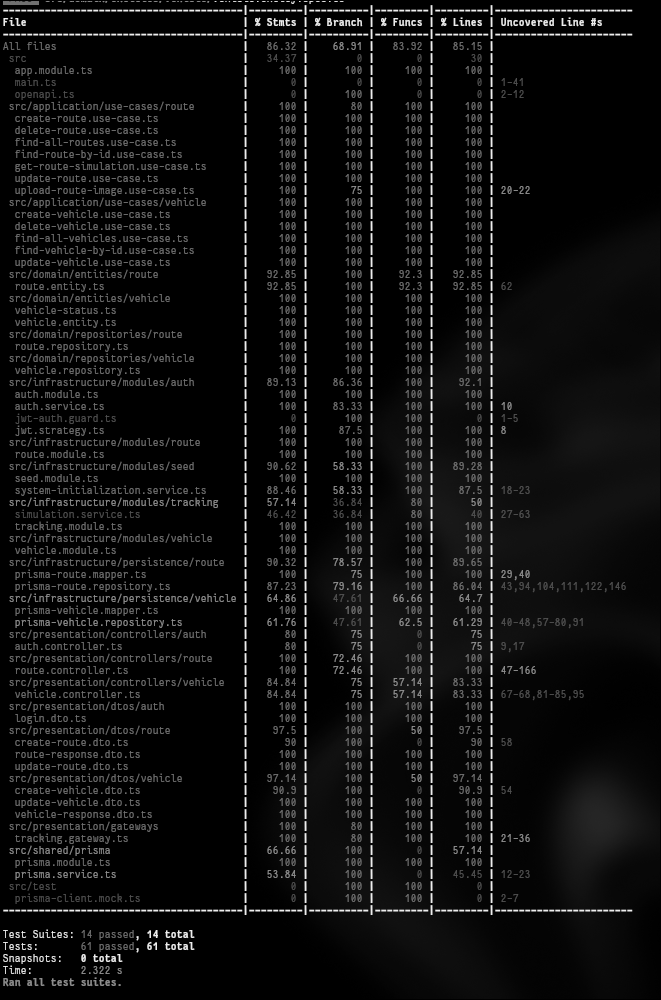
\includegraphics[width=0.85\textwidth]{assets/captura-cobertura-pruebas.png}
    \figcaptionwithauthor{Reporte de cobertura de código (Code Coverage) de las pruebas en el Backend}
\end{figure}

\paragraph{Pruebas de DevOps y Despliegue (VPS, Traefik y Let's Encrypt)}
La validación de la infraestructura en producción (VPS Linux) se orientó a la estabilidad del canal de comunicación bidireccional de WebSockets y a la robustez del flujo automático de Integración y Despliegue Continuo (CI/CD) orquestado a través de \textbf{GitHub Actions}.

El pipeline de entrega continua está diseñado bajo dos flujos de trabajo paralelos y automáticos:
\begin{itemize}
    \item \textbf{Integración Continua (CI):} Se ejecuta en cada Push o Pull Request hacia la rama \texttt{develop}. En el \textbf{Backend}, este flujo inicializa un entorno virtual de Node.js, instala las dependencias de forma consistente mediante \texttt{pnpm install --frozen-lockfile}, genera el cliente de base de datos de Prisma (\texttt{prisma:generate}), valida la calidad estática de sintaxis y tipado (\texttt{pnpm lint}), ejecuta la suite completa de pruebas unitarias con Jest (\texttt{pnpm test}) y finalmente compila el código en producción (\texttt{pnpm build}). En el \textbf{Frontend}, el flujo análogo asegura que la interfaz de usuario basada en Next.js compile su empaquetado de producción de forma limpia y pase la auditoría estática de ESLint.
    \begin{figure}[H]
        \centering
        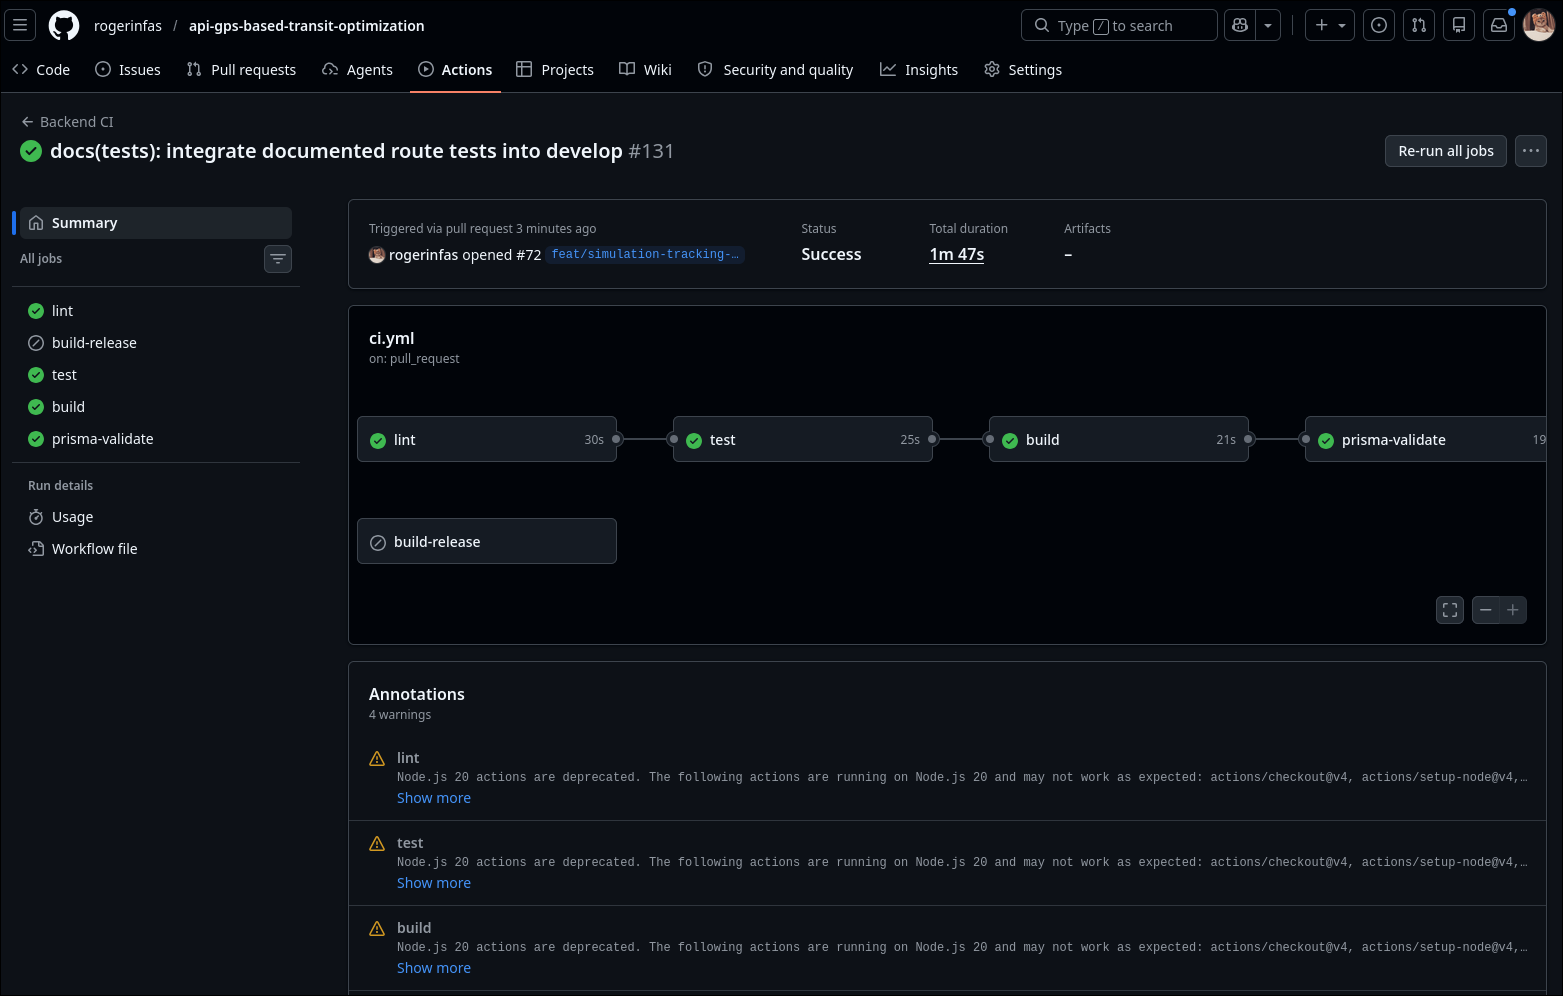
\includegraphics[width=1\textwidth]{assets/captura-ci-backend.png}
        \figcaptionwithauthor{Flujo de Integración Continua (CI) del Backend en GitHub Actions}
    \end{figure}

    \begin{figure}[H]
        \centering
        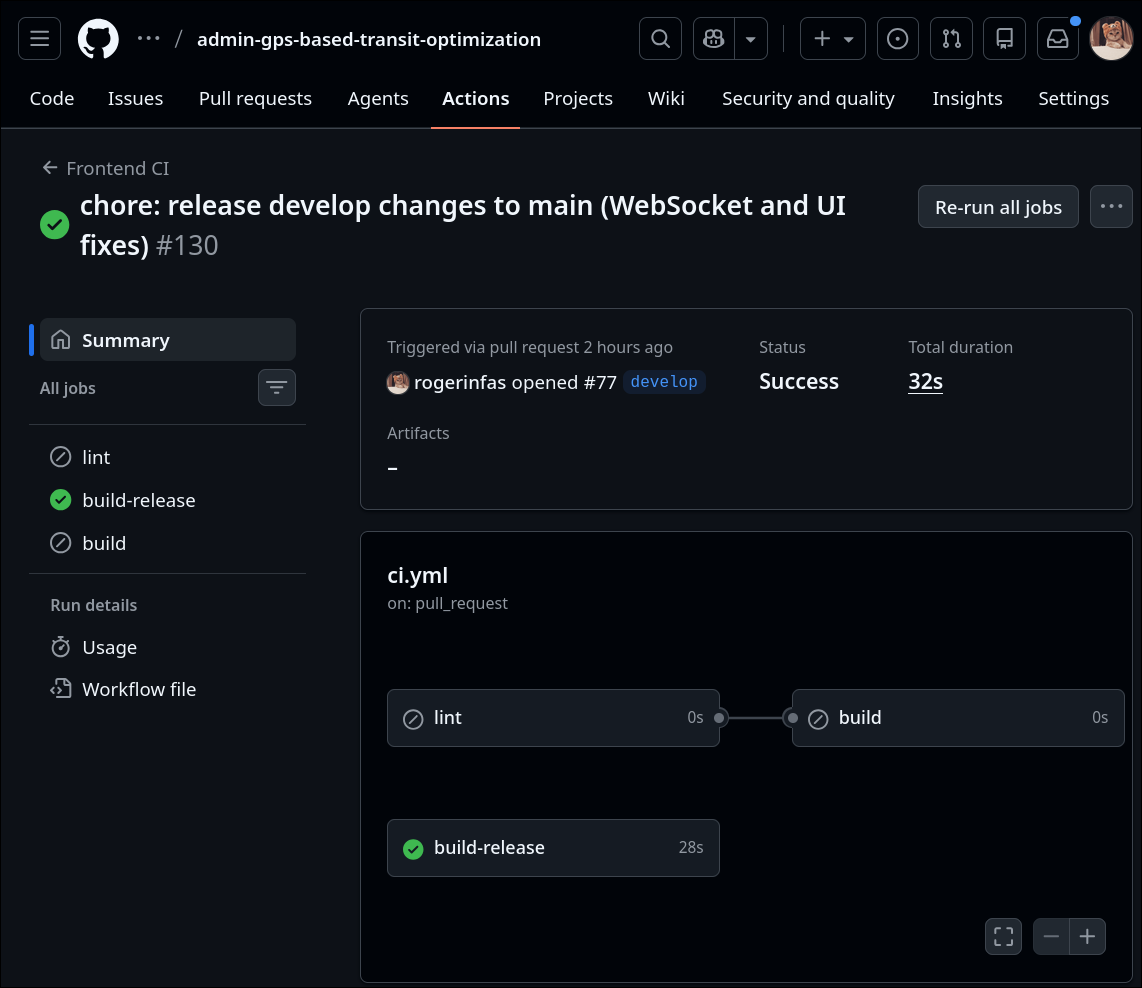
\includegraphics[width=1\textwidth]{assets/captura-ci-frontend.png}
        \figcaptionwithauthor{Flujo de Integración Continua (CI) del Frontend en GitHub Actions}
    \end{figure}

    \item \textbf{Despliegue Continuo (CD):} Se activa automáticamente tras la aprobación e integración de los cambios en las ramas principales de producción (\texttt{main}/\texttt{master}). GitHub Actions establece una conexión segura mediante SSH Key secreta al servidor VPS, sincroniza el código remoto, construye las imágenes optimizadas de Docker multi-stage y orquesta el reinicio seguro de los contenedores mediante \texttt{docker-compose.prod.yml}. Este despliegue aplica automáticamente las migraciones pendientes en PostgreSQL (\texttt{prisma migrate deploy}) y levanta el servicio por detrás del proxy inverso de \textbf{Traefik}, el cual asigna automáticamente los certificados SSL de \textbf{Let's Encrypt} y activa las Sticky Sessions.
\end{itemize}

\begin{figure}[H]
    \centering
    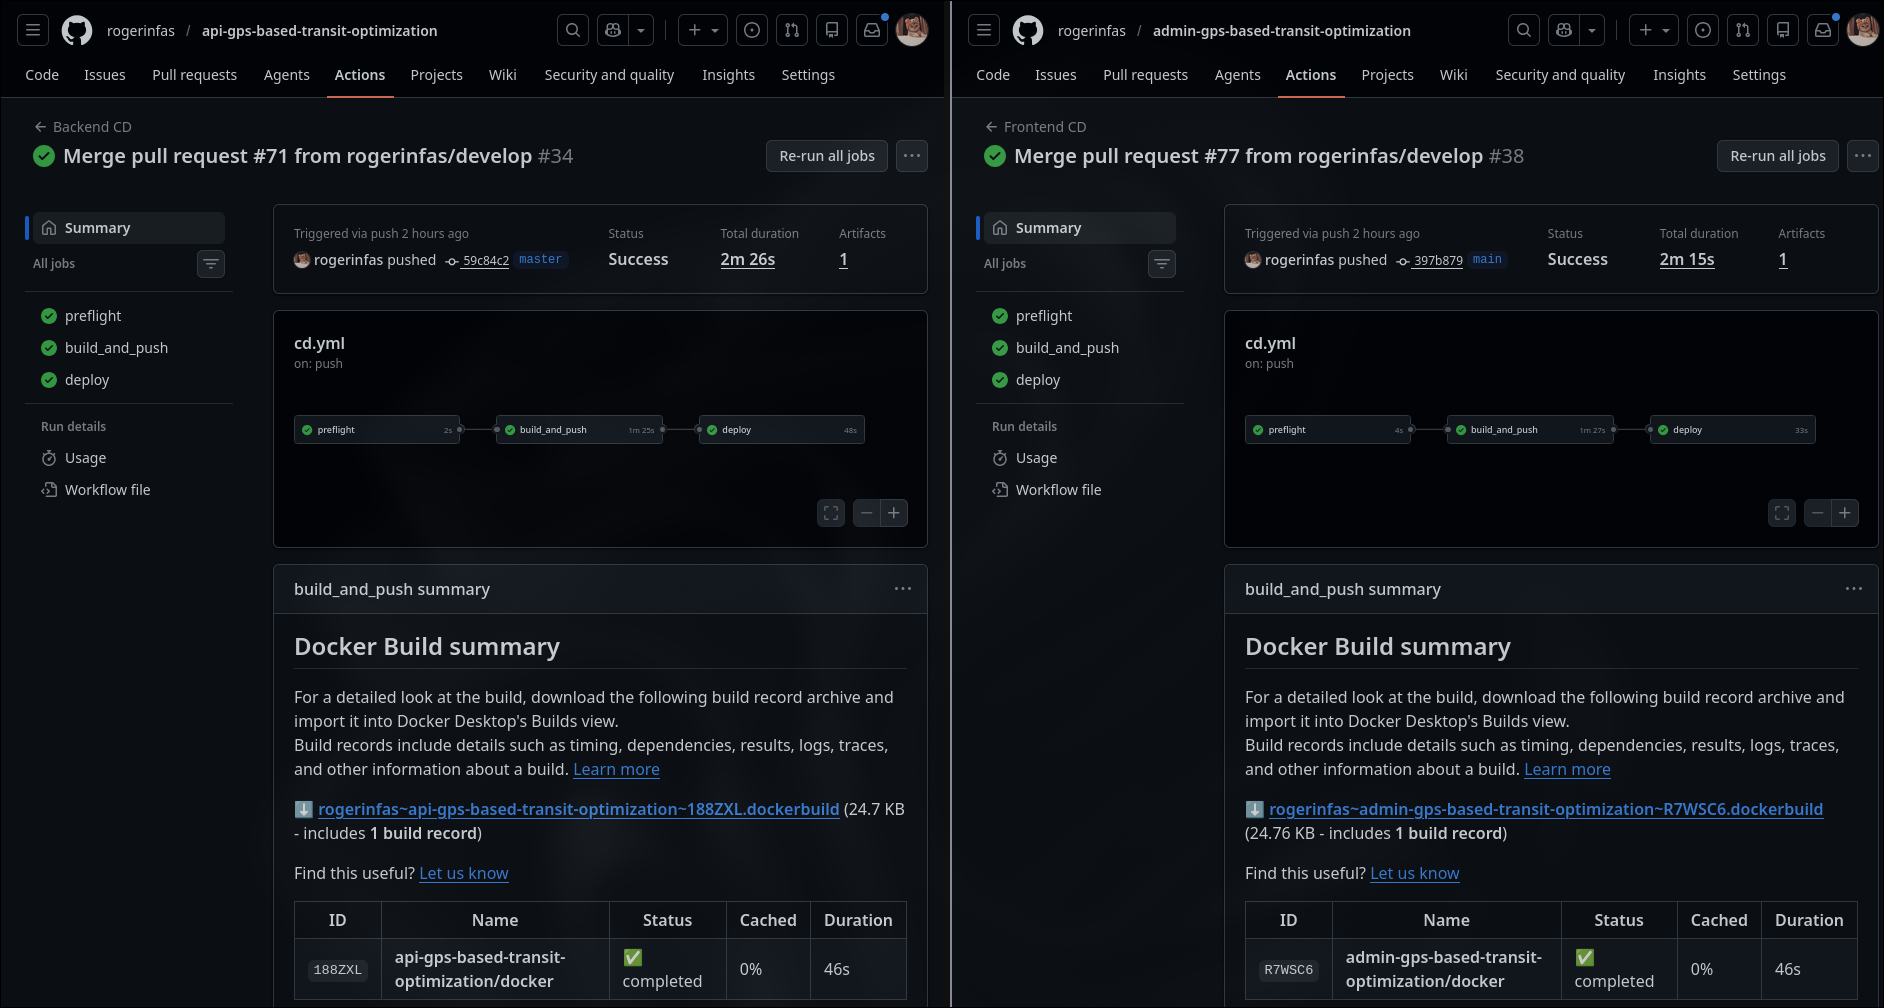
\includegraphics[width=1\textwidth]{assets/captura-cd-despliegue.png}
    \figcaptionwithauthor{Orquestación conjunta del Despliegue Continuo (CD) de Frontend y Backend en el servidor de producción desde Github Actions}
\end{figure}

Para validar y verificar la estabilidad operativa del entorno de producción directamente en el servidor VPS, se implementó el monitoreo activo de contenedores mediante la herramienta \textbf{ctop}. Esta interfaz gráfica por terminal permite inspeccionar en tiempo real el consumo de recursos (CPU, memoria, red y disco) de cada servicio orquestado en Docker. 

En la Figura \ref{fig:ctop-general} se observa el listado general del estado saludable y en ejecución de todos los contenedores que componen la infraestructura (incluyendo el proxy inverso \textbf{Traefik}, la base de datos centralizada de producción \textbf{PostgreSQL}, el servicio del \textbf{Backend} y la aplicación del \textbf{Frontend}). De igual manera, en la Figura \ref{fig:ctop-detalle} se visualiza la telemetría detallada del contenedor del backend, constatando un consumo mínimo de recursos y un correcto comportamiento de las conexiones a sockets.

\begin{figure}[H]
    \centering
    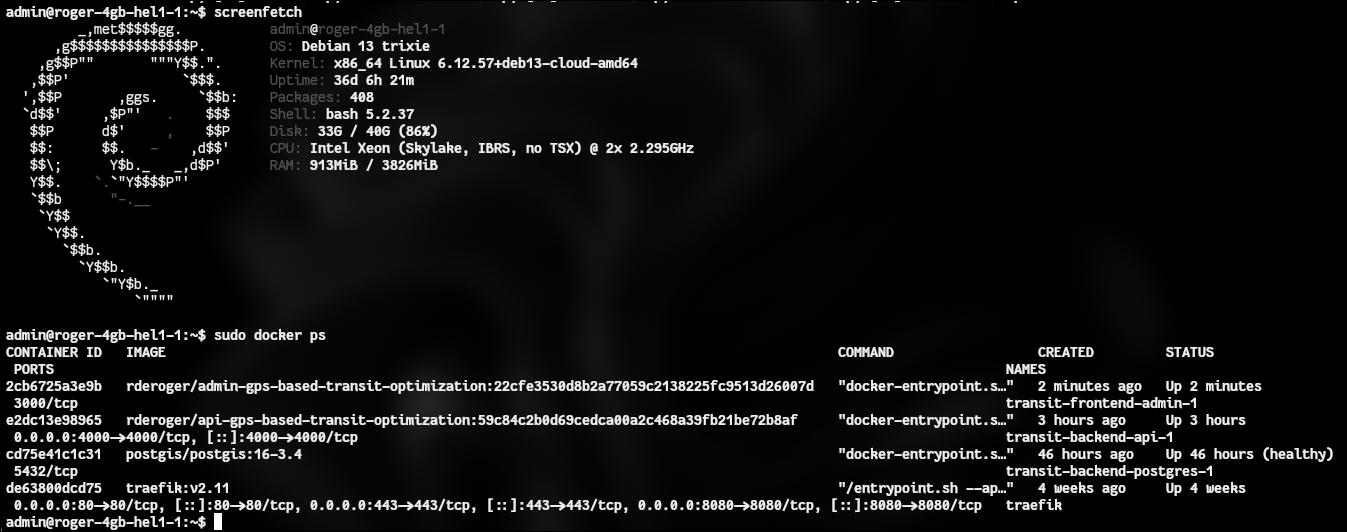
\includegraphics[width=1\textwidth]{assets/captura-ctop-general.png}
    \figcaptionwithauthor{Monitoreo general de los contenedores Docker en ejecución activa dentro del VPS de producción mediante la interfaz de terminal ctop}
    \label{fig:ctop-general}
\end{figure}

\begin{figure}[H]
    \centering
    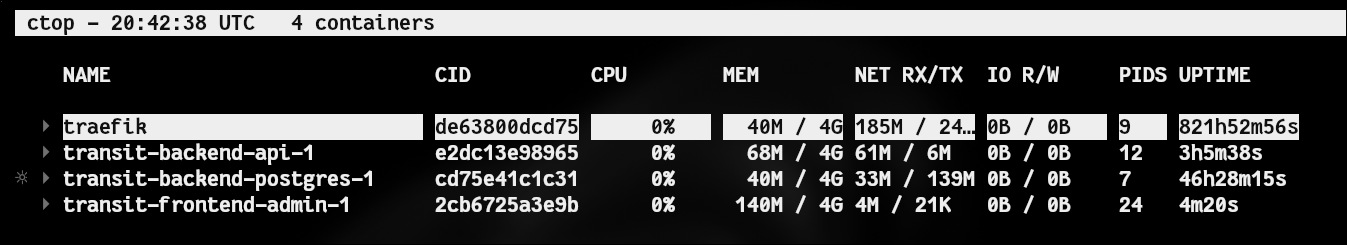
\includegraphics[width=1\textwidth]{assets/captura-ctop-detalle.png}
    \figcaptionwithauthor{Inspección detallada del contenedor Docker correspondiente al backend del sistema en producción en ctop}
    \label{fig:ctop-detalle}
\end{figure}

\paragraph{Pruebas de Diseño de Interfaz y UI/UX (Frontend)}
El panel web administrador y de monitoreo de usuario final fue verificado en base a las siguientes dimensiones funcionales:
\begin{itemize}
    \item \textbf{Responsividad y Usabilidad:} La interfaz web basada en componentes reactivos de React 19 y Tailwind CSS 4 responde fluidamente a dispositivos móviles y escritorios, asegurando que el mapa interactivo ocupe el área correcta y los menús de filtrado de rutas sean totalmente accesibles. Para validar la correcta adaptación y visualización adaptativa (responsividad) en múltiples pantallas concurrentemente, se utilizó la extensión de Google Chrome \textbf{Responsive Viewer}, evaluando los layouts operativos en resoluciones críticas equivalentes a un iPhone 14, iPhone 14 Pro Max, iPad Air 5 y MacBook Air.
    \begin{figure}[H]
    \centering
    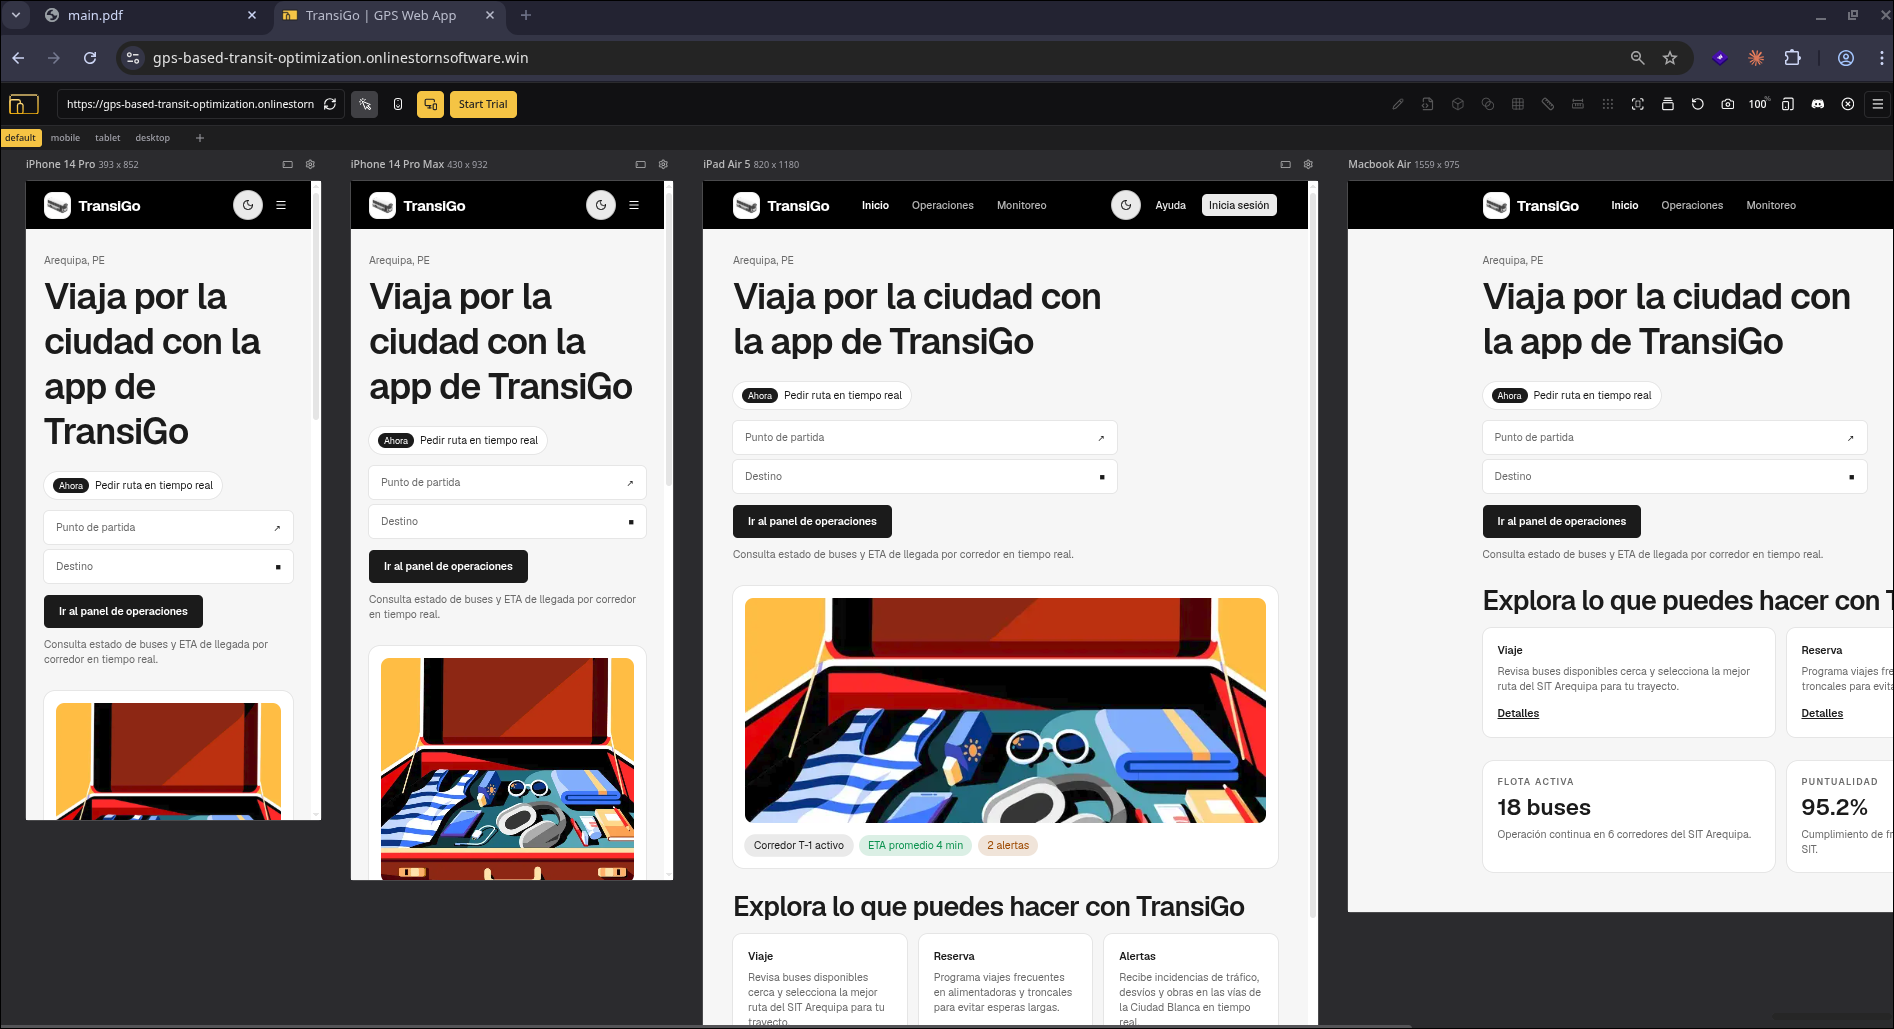
\includegraphics[width=\textwidth]{assets/captura-responsive-viewer.png}
    \figcaptionwithauthor{Validación de responsividad multidispositivo de la pantalla de monitoreo principal (iPhone 14, iPhone 14 Pro Max, iPad Air 5 y MacBook Air) mediante la herramienta Responsive Viewer}
    \end{figure}

    \begin{figure}[H]
        \centering
        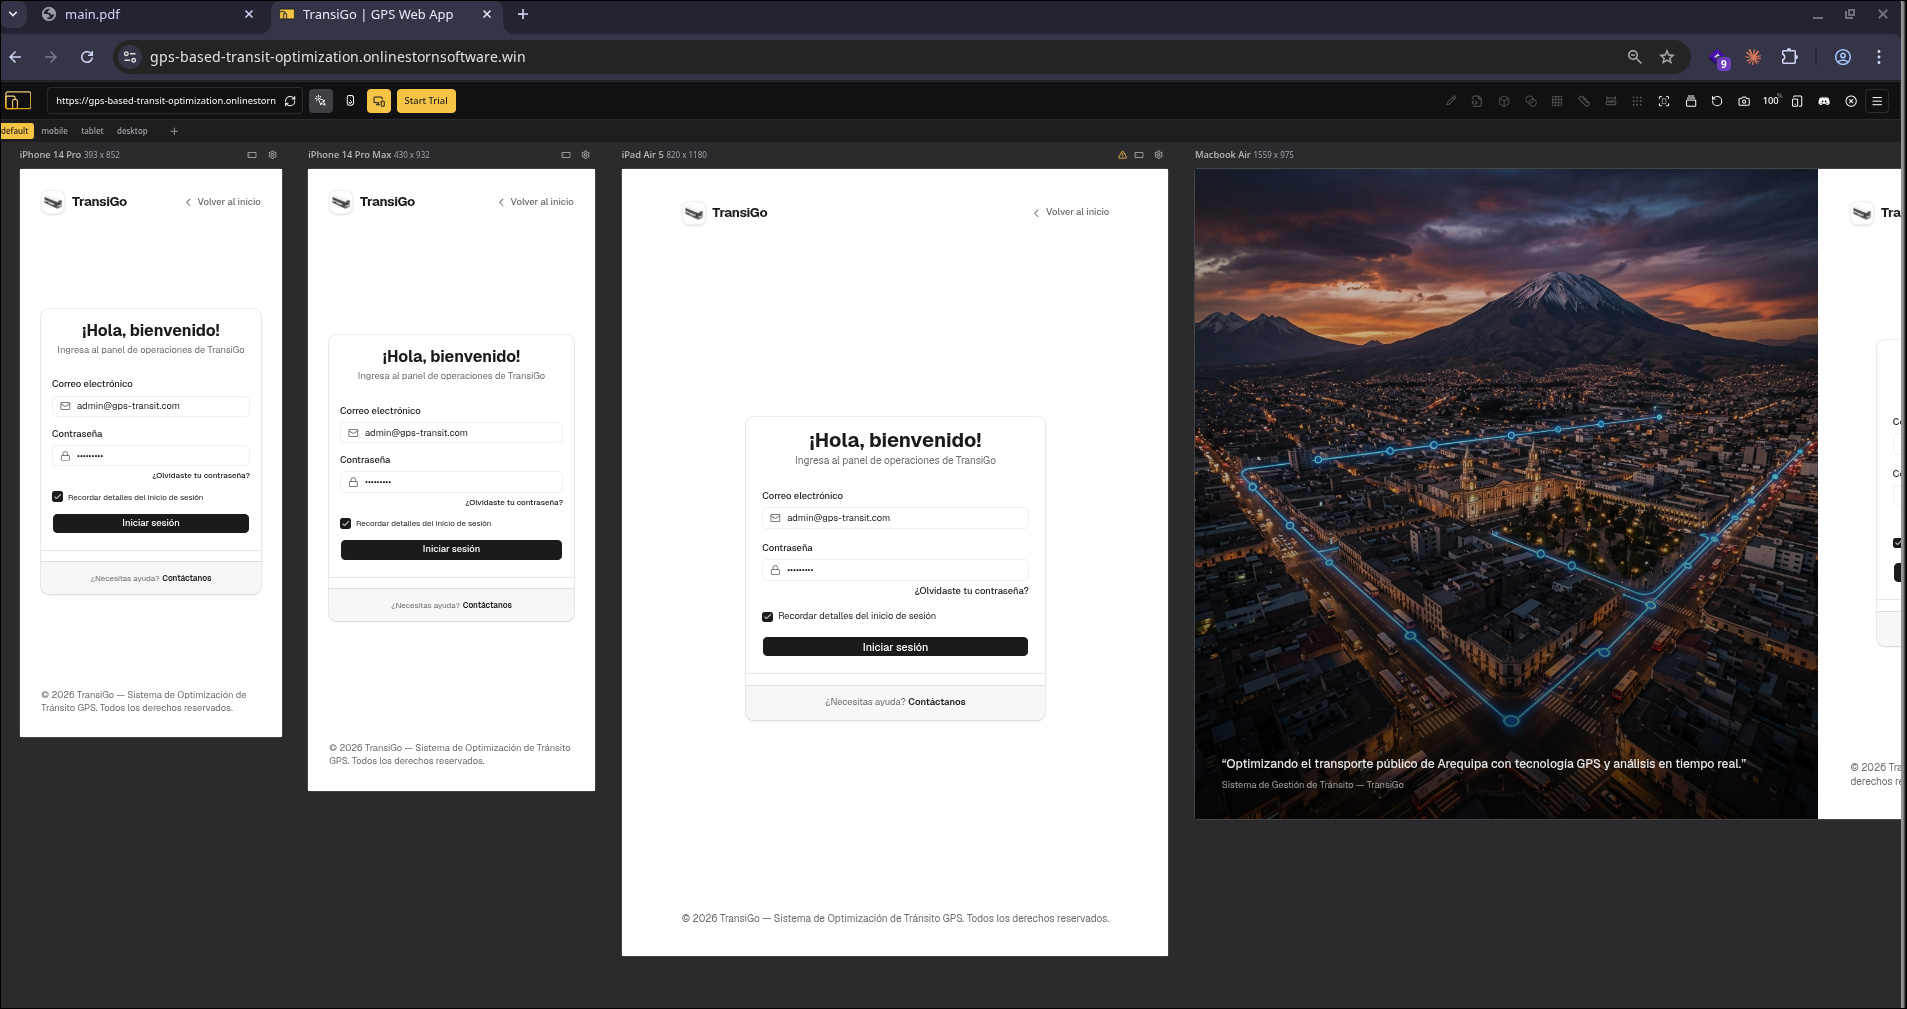
\includegraphics[width=\textwidth]{assets/captura-responsive-login.png}
        \figcaptionwithauthor{Validación de responsividad multidispositivo de la interfaz de inicio de sesión (Login) mediante la herramienta Responsive Viewer}
    \end{figure}

    \begin{figure}[H]
        \centering
        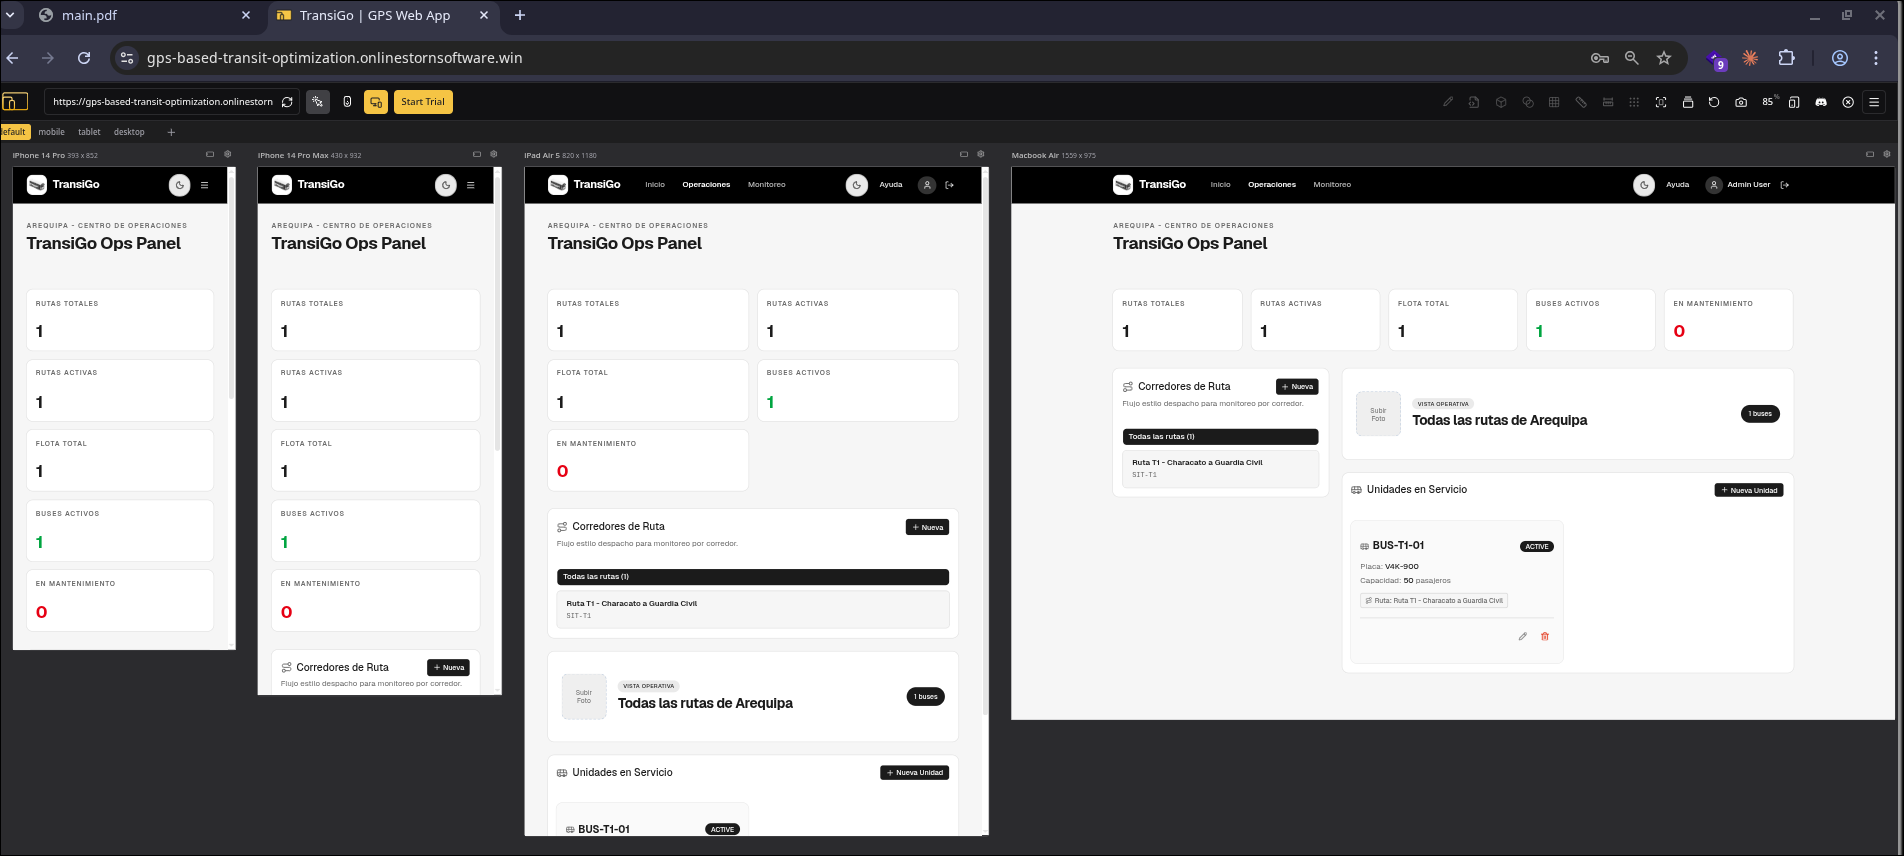
\includegraphics[width=\textwidth]{assets/captura-responsive-operations.png}
        \figcaptionwithauthor{Validación de responsividad multidispositivo del panel de operaciones administrativas mediante la herramienta Responsive Viewer}
    \end{figure}

    \begin{figure}[H]
        \centering
        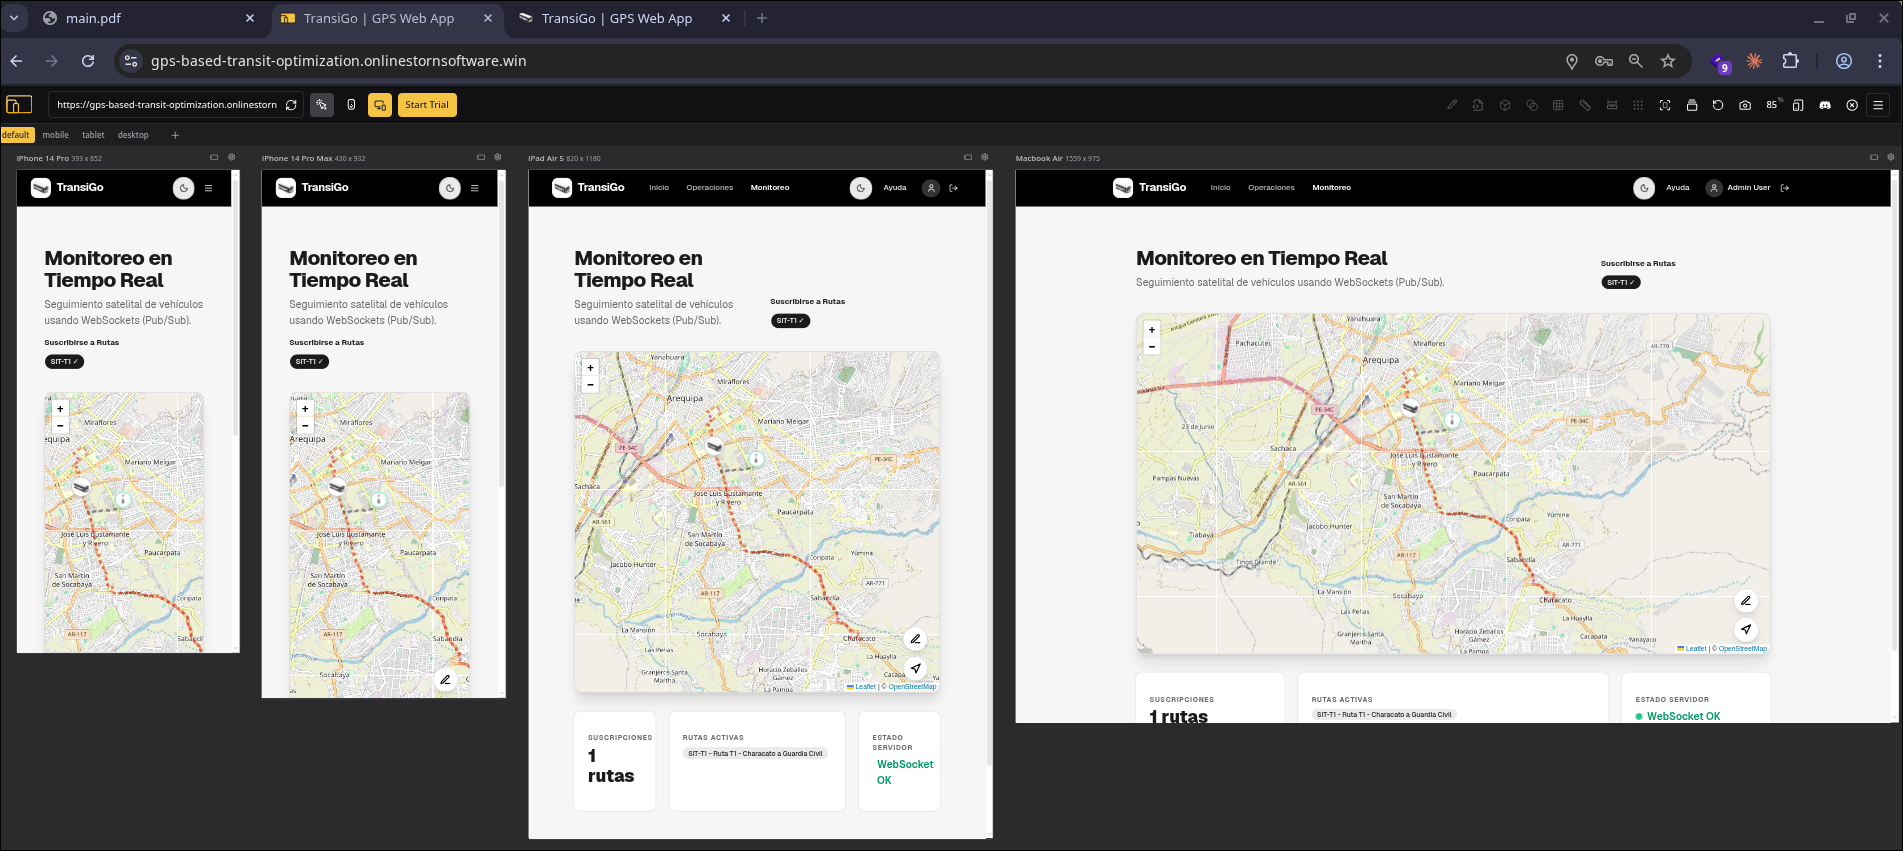
\includegraphics[width=\textwidth]{assets/captura-responsive-simulation.png}
        \figcaptionwithauthor{Validación de responsividad multidispositivo del panel de monitoreo y simulación geoespacial en tiempo real (\texttt{/simulation}) mediante la herramienta Responsive Viewer}
    \end{figure}

        \item \textbf{Monitoreo Geoespacial Activo:} Pruebas dinámicas con la API espacial de \textbf{Leaflet} comprobando el correcto dibujado del trazado en mapa de la geometría \texttt{LineString} de las rutas SIT y la actualización reactiva instantánea de los marcadores de posición de buses mediante las suscripciones a salas en tiempo real de WebSockets.
    \end{itemize}

\paragraph{Validación Estadística de Hipótesis (Prueba de Wilcoxon)}

Para evaluar formalmente el impacto de la plataforma de monitoreo web y tracking GPS sobre el tiempo de espera de los usuarios, se diseñó un experimento con un tamaño de muestra $N = 20$ usuarios recurrentes de los corredores del SIT. El estudio comparó los tiempos de espera registrados en dos escenarios:
\begin{enumerate}
    \item \textbf{Pre-test (Sin GPS):} Tiempo de espera de los usuarios en minutos acudiendo al paradero bajo el esquema tradicional de operación (sin información del arribo de los buses).
    \item \textbf{Post-test (Con GPS):} Tiempo de espera de los mismos usuarios utilizando la aplicación web de telemetría y consulta de ETA en tiempo real, permitiéndoles acudir al paradero de forma sincronizada con el arribo de las unidades.
\end{enumerate}

Para asegurar la rigurosidad estadística en la elección de la prueba de contraste, primero se aplicó el test de normalidad de \textbf{Shapiro-Wilk} a ambos grupos de mediciones. La prueba de Shapiro-Wilk arrojó un valor $p = 0.3608$ para el Pre-test (indicando normalidad) y $p = 0.0205$ para el Post-test (rechazando la normalidad al ser $p < 0.05$). Al no cumplirse el supuesto de normalidad en ambas distribuciones de manera conjunta, se invalida el uso de pruebas paramétricas como la prueba \textit{t de Student} para muestras pareadas, justificando la aplicación obligatoria de la prueba no paramétrica de \textbf{Rangos con Signo de Wilcoxon}.

A continuación, se formulan las hipótesis estadísticas correspondientes:
\begin{itemize}
    \item \textbf{Hipótesis Nula ($H_0$):} La mediana de las diferencias de los tiempos de espera entre el pre-test y el post-test es igual a cero (el sistema GPS no produce ninguna reducción en la espera).
    $$H_0: \tilde{\theta}_{pre} = \tilde{\theta}_{post}$$
    \item \textbf{Hipótesis Alternativa ($H_1$):} La mediana de los tiempos de espera de los usuarios en el post-test es menor en comparación con el pre-test (el sistema GPS reduce significativamente la espera).
    $$H_1: \tilde{\theta}_{pre} > \tilde{\theta}_{post}$$
\end{itemize}

Los estadísticos descriptivos calculados a partir de los datos experimentales se resumen en la Tabla \ref{tab:descriptivos_wilcoxon}.

\begin{table}[H]
\centering
\caption{Estadísticos descriptivos y resultados de normalidad (N=20)}
\label{tab:descriptivos_wilcoxon}
\resizebox{\textwidth}{!}{%
\begin{tabular}{|l|c|c|c|c|c|c|}
\hline
\rowcolor[HTML]{F3F4F6} 
\textbf{Grupo} & \textbf{Media (min)} & \textbf{Mediana (min)} & \textbf{Desv. Est.} & \textbf{Mínimo} & \textbf{Máximo} & \textbf{Shapiro-Wilk (p)} \\ \hline
Pre-test (Sin GPS) & 15.27 & 14.80 & 3.86 & 9.50 & 24.50 & 0.3608 \\ \hline
Post-test (Con GPS) & 8.05 & 7.65 & 1.64 & 5.70 & 13.20 & 0.0205 \\ \hline
\end{tabular}%
}
\figcaptionwithauthor{Estadísticas descriptivos del experimento de tiempos de espera}
\end{table}

Como se observa, se experimentó una notable reducción en la media de los tiempos de espera, pasando de $15.27$ minutos (Pre-test) a $8.05$ minutos (Post-test), lo cual equivale a una disminución promedio del $47.28\%$. La dispersión de los datos (desviación estándar) también se redujo drásticamente de $3.86$ a $1.64$ minutos, indicando un servicio de espera mucho más predecible y homogéneo para los usuarios.

La distribución de los tiempos de espera se visualiza gráficamente en la Figura \ref{fig:fig-wilcoxon}, donde se aprecian con claridad los cuartiles y la reducción de la variabilidad extrema.

\begin{figure}[H]
\centering
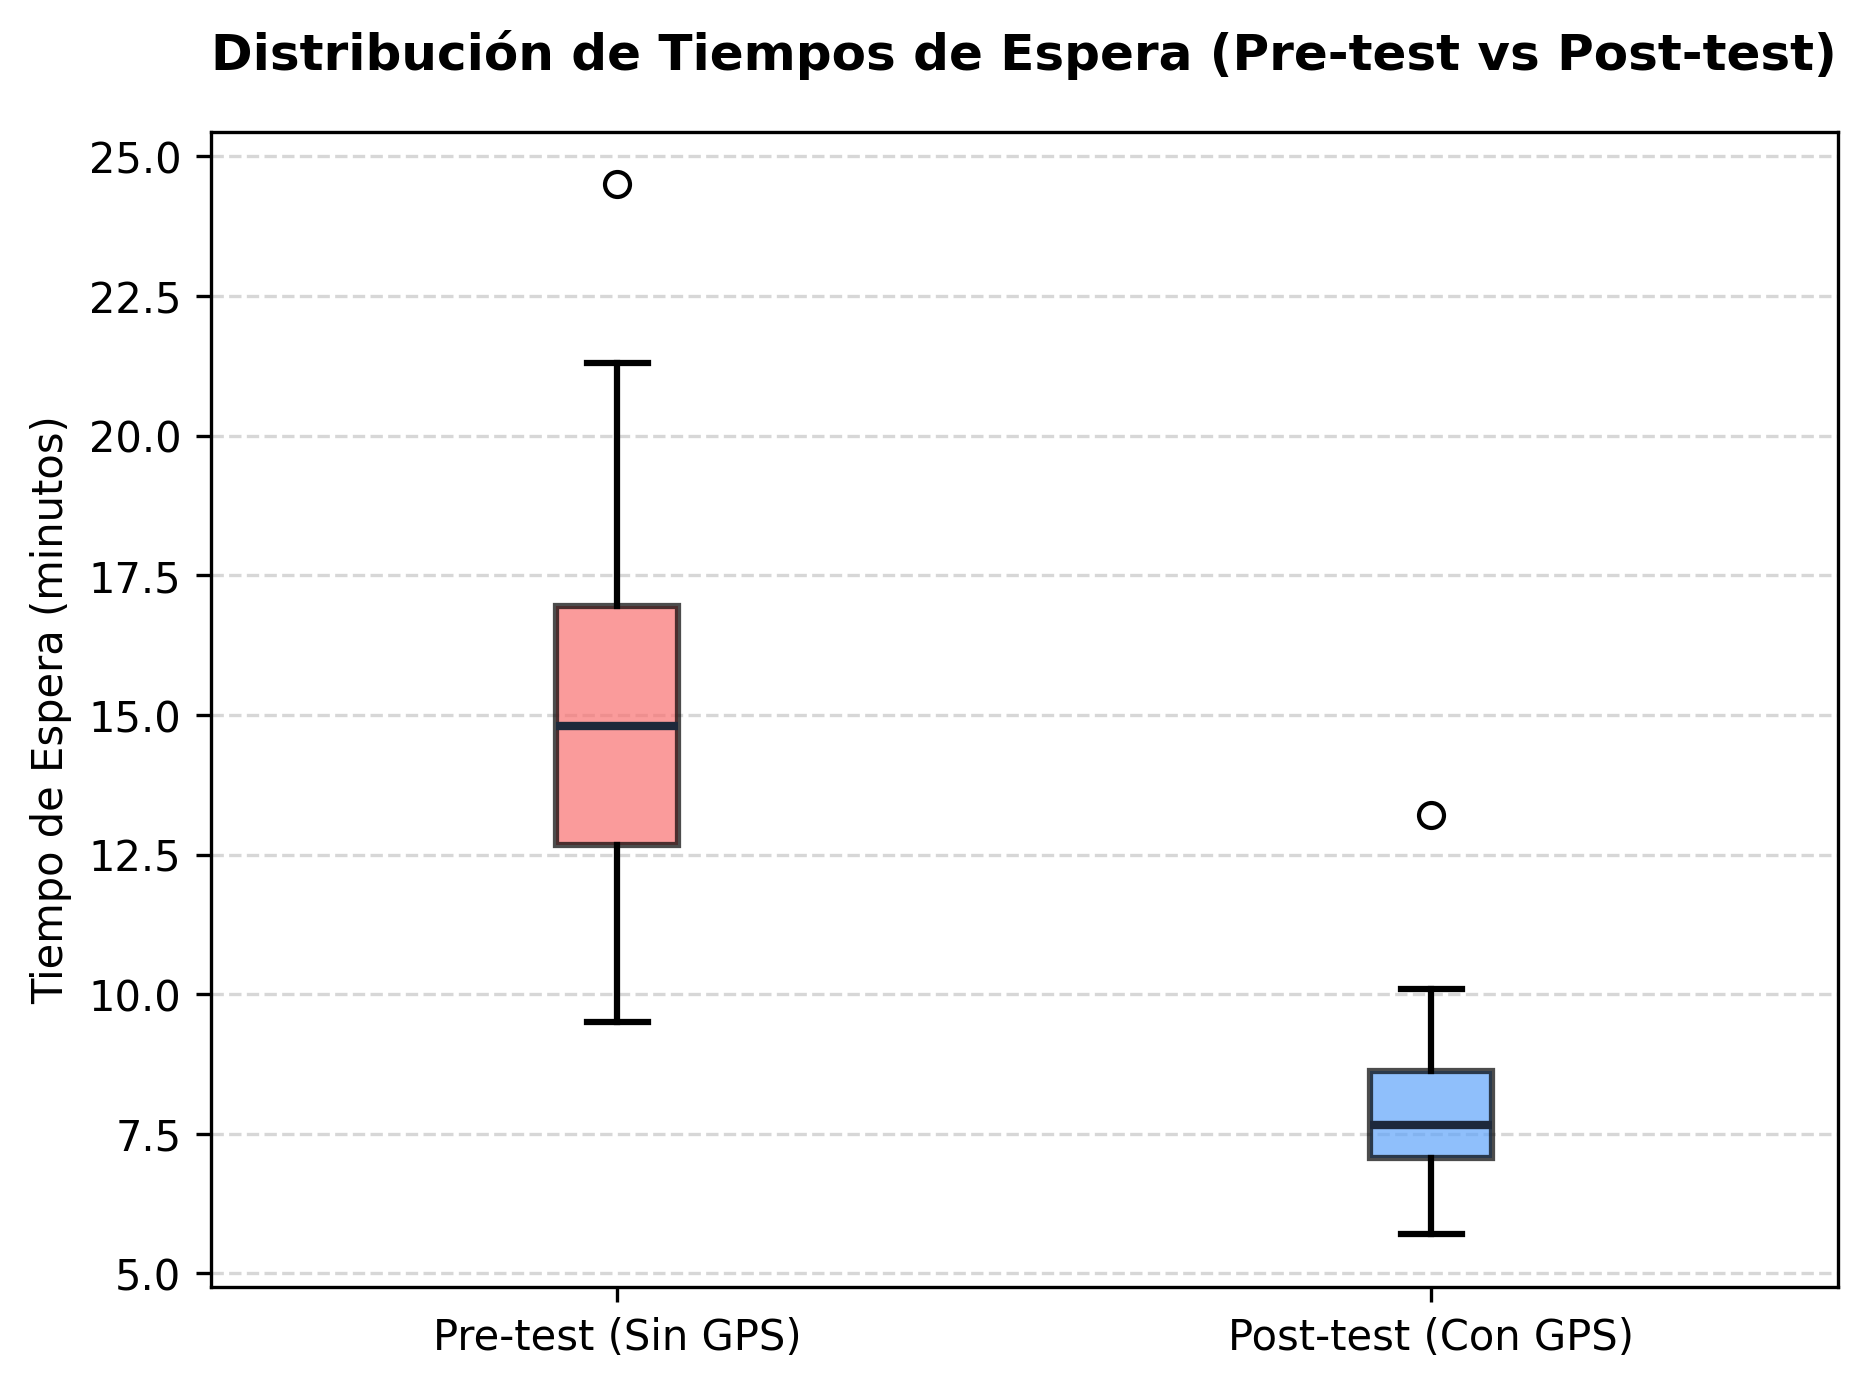
\includegraphics[width=0.75\textwidth]{assets/grafico-wilcoxon.png}
\figcaptionwithauthor{Distribución comparativa de tiempos de espera mediante diagrama de cajas (Boxplot)}
\label{fig:fig-wilcoxon}
\end{figure}

A continuación, se detalla de manera rigurosa y procedimental la aplicación del algoritmo de la Prueba de Rangos con Signo de Wilcoxon para muestras relacionadas sobre las 20 observaciones pareadas, garantizando la trazabilidad matemática y la validación formal de los resultados por parte de los revisores académicos:

\begin{enumerate}
    \item \textbf{Paso 1: Cálculo de Diferencias.} Para cada sujeto de la muestra, se toma el valor del tiempo de espera de la Condición 1 (Pre-test) y se le resta el valor correspondiente de la Condición 2 (Post-test) para obtener la diferencia real $d_i = X_{1,i} - X_{2,i}$.
    \item \textbf{Paso 2: Filtrado de Ceros.} Se revisa la lista de diferencias y se descartan los valores exactamente iguales a cero ($d_i = 0$). En este experimento, ninguna de las 20 diferencias resultó nula, por lo que la muestra efectiva para el test estadístico se mantiene en $N' = 20$.
    \item \textbf{Paso 3: Ordenamiento de Valores Absolutos.} Se calcula el valor absoluto de las diferencias $|d_i|$, ignorando temporalmente su signo, y se ordenan de menor a mayor. A cada observación se le asigna una posición de orden consecutiva (caja de orden) desde la posición 1 hasta la 20.
    \item \textbf{Paso 4: Tratamiento de Empates (Promedios).} En los casos donde existen valores absolutos idénticos que ocupan múltiples posiciones consecutivas, se calcula la media aritmética de dichas posiciones. Dicho promedio se asigna como el rango final para todas las observaciones empatadas en ese valor.
    \item \textbf{Paso 5: Asignación de Signos.} A cada rango final calculado se le restituye el signo ($+$ o $-$) que tenía la diferencia original en el Paso 1. Dado que todas las diferencias calculadas en este experimento son positivas ($d_i > 0$), todos los rangos asignados reciben signo positivo ($+$).
    \item \textbf{Paso 6: Sumatorias por Signo.} Se realizan las sumas independientes de las posiciones correspondientes a cada signo:
    \begin{itemize}
        \item Suma de rangos positivos ($W^+$):
        $$W^+ = \sum_{d_i > 0} R_i = 1.0 + 2.0 + 3.0 + \dots + 20.0 = 210.0$$
        \item Suma de rangos negativos ($W^-$):
        $$W^- = \sum_{d_i < 0} R_i = 0.0$$
    \end{itemize}
    \item \textbf{Paso 7: Estadístico W.} Se define el estadístico $W$ de Wilcoxon como la sumatoria de menor valor numérico entre ambas:
    $$W = \min(W^+, W^-) = \min(210.0, 0.0) = 0.0$$
    \item \textbf{Paso 8: Regla de Decisión y Valor Crítico.} Dado que planteamos una hipótesis unilateral de una cola (buscando determinar si el sistema reduce el tiempo de espera), el nivel de significancia de $\alpha = 0.05$ se evalúa de manera directa. Para una muestra de tamaño $N' = 20$ en una prueba de una cola, el valor crítico tabulado es $W_{\text{crit}} = 60$ (y para una prueba de dos colas con $\alpha/2=0.025$ es $W_{\text{crit}} = 52$). La hipótesis nula $H_0$ se rechaza si el estadístico calculado es menor o igual al valor crítico:
    $$W_{\text{calc}} = 0.0 \le W_{\text{crit}} = 60 \implies \text{Se rechaza la hipótesis nula } H_0$$
\end{enumerate}

El desglose matemático detallado para cada una de las 20 observaciones pareadas, con la asignación correspondiente de diferencias, valores absolutos, rangos consecutivos y promedios de empates, se expone de forma exhaustiva en la Tabla \ref{tab:wilcoxon_paso_a_paso}.

\begin{table}[H]
\centering
\caption{Cálculo paso a paso de rangos para la Prueba de Wilcoxon (N=20)}
\label{tab:wilcoxon_paso_a_paso}
\resizebox{\textwidth}{!}{%
\begin{tabular}{|c|c|c|c|c|c|c|c|c|}
\hline
\rowcolor[HTML]{F3F4F6} 
\textbf{ID} & \textbf{Pre-test ($X_1$)} & \textbf{Post-test ($X_2$)} & \textbf{Dif. ($d_i$)} & \textbf{Abs. ($|d_i|$)} & \textbf{Caja Temp.} & \textbf{Rango Final} & \textbf{Signo} & \textbf{Rango Signado} \\ \hline
1 & 14.9 & 13.2 & 1.7 & 1.7 & 1 & 1.0 & + & 1.0 \\ \hline
2 & 14.7 & 6.1 & 8.6 & 8.6 & 15 & 15.0 & + & 15.0 \\ \hline
3 & 13.4 & 7.5 & 5.9 & 5.9 & 9 & 9.0 & + & 9.0 \\ \hline
4 & 9.5 & 6.6 & 2.9 & 2.9 & 3 & 3.0 & + & 3.0 \\ \hline
5 & 12.9 & 7.8 & 5.1 & 5.1 & 8 & 8.0 & + & 8.0 \\ \hline
6 & 10.1 & 7.0 & 3.1 & 3.1 & 4 & 4.0 & + & 4.0 \\ \hline
7 & 16.6 & 8.2 & 8.4 & 8.4 & 13 & 13.5 & + & 13.5 \\ \hline
8 & 13.4 & 7.1 & 6.3 & 6.3 & 10 & 10.0 & + & 10.0 \\ \hline
9 & 16.9 & 8.5 & 8.4 & 8.4 & 14 & 13.5 & + & 13.5 \\ \hline
10 & 17.1 & 10.1 & 7.0 & 7.0 & 11 & 11.0 & + & 11.0 \\ \hline
11 & 11.8 & 7.5 & 4.3 & 4.3 & 6 & 6.0 & + & 6.0 \\ \hline
12 & 17.6 & 7.4 & 10.2 & 10.2 & 16 & 16.0 & + & 16.0 \\ \hline
13 & 15.7 & 8.4 & 7.3 & 7.3 & 12 & 12.0 & + & 12.0 \\ \hline
14 & 12.0 & 8.1 & 3.9 & 3.9 & 5 & 5.0 & + & 5.0 \\ \hline
15 & 24.5 & 7.4 & 17.1 & 17.1 & 20 & 20.0 & + & 20.0 \\ \hline
16 & 21.3 & 6.9 & 14.4 & 14.4 & 19 & 19.0 & + & 19.0 \\ \hline
17 & 16.9 & 5.7 & 11.2 & 11.2 & 17 & 17.0 & + & 17.0 \\ \hline
18 & 11.6 & 9.1 & 2.5 & 2.5 & 2 & 2.0 & + & 2.0 \\ \hline
19 & 13.5 & 9.0 & 4.5 & 4.5 & 7 & 7.0 & + & 7.0 \\ \hline
20 & 21.0 & 9.4 & 11.6 & 11.6 & 18 & 18.0 & + & 18.0 \\ \hline
\end{tabular}%
}
\figcaptionwithauthor{Desglose del cálculo de rangos para la Prueba de Wilcoxon}
\end{table}

Al ejecutar el contraste general, se obtuvieron los resultados consolidados en la Tabla \ref{tab:resultado_wilcoxon}.

\begin{table}[H]
\centering
\caption{Resultados de la prueba de Wilcoxon (Muestras Relacionadas)}
\label{tab:resultado_wilcoxon}
\resizebox{\textwidth}{!}{%
\begin{tabular}{|l|c|c|c|c|}
\hline
\rowcolor[HTML]{F3F4F6} 
\textbf{Comparación} & \textbf{Suma Rangos ($W^+$)} & \textbf{Suma Rangos ($W^-$)} & \textbf{Estadístico $W$} & \textbf{p-valor} \\ \hline
Pre-test > Post-test & 210.0 & 0.0 & 0.0 & 9.54e-07 \\ \hline
\end{tabular}%
}
\figcaptionwithauthor{Resultados de la prueba de rangos con signo de Wilcoxon}
\end{table}

Dado que el estadístico obtenido ($W = 0.0$) es menor que el valor crítico de una cola para $N=20$ ($\alpha=0.05 \implies W_{\text{crit}} = 60$) y el valor de probabilidad obtenido ($p = 9.54 \times 10^{-7}$) es sustancialmente menor que el nivel de significancia prefijado $\alpha = 0.05$ (e incluso menor que $\alpha = 0.001$), se \textbf{rechaza categóricamente la hipótesis nula ($H_0$)} en favor de la hipótesis alternativa ($H_1$). Se concluye de manera contundente que el uso del sistema de optimización y monitoreo de rutas de transporte basado en posicionamiento global reduce significativamente los tiempos de espera de los pasajeros en el área metropolitana de Arequipa.


\subsubsection{Mantenimiento}

Esta sección documentará las actividades de ajuste, mejora y sostenibilidad de la solución, incluyendo control de cambios, correcciones y recomendaciones para evolución futura.

\begin{itemize}
    \item Registro de mejoras posteriores a pruebas: \textbf{(vacío por ahora)}.
    \item Control de versiones y cambios relevantes: \textbf{(vacío por ahora)}.
    \item Recomendaciones de evolución tecnológica: \textbf{(vacío por ahora)}.
    \item Consideraciones de operación continua: \textbf{(vacío por ahora)}.
\end{itemize}

